% criação do documento com a classe abntex2
\documentclass[a4paper,
               article,
               12pt,
               openany,
               oneside,
               english,
               brazil]{abntex2}

% pacotes
\usepackage{fontspec}
\usepackage{times}			    % usa a fonte Latin Modern
\usepackage[T1]{fontenc}		% seleção de códigos de fonte.
\usepackage[utf8]{inputenc}		% codificação do documento (conversão automática dos acentos)
\usepackage{indentfirst}		% indenta o primeiro parágrafo de cada seção.
\usepackage{color}		        % controle das cores
\usepackage{graphicx}			% inclusão de gráficos/figuras.
\usepackage{subcaption}			% inclusão de subfiguras.
\usepackage{microtype} 			% para melhorias de justificação
\usepackage{amsmath}			% pacote matemático
\usepackage[brazil]{babel}      % pacote multilinguagem
\usepackage{fancyhdr}           % cabeçalhos etc.
\usepackage{array}
\usepackage{url}
\urlstyle{same}
% \usepackage[alf]{abntex2cite}   % citações abnt
\usepackage[backend=biber, style=abnt, justify]{biblatex}
\addbibresource{../bibliografia.bib}

% cabeçalho
\fancyhead{}
\rhead{\thepage}
\cfoot{}

\pretextual
\autor{Phelipe Teles da Silva}
\titulo{Determinantes macroeconômicos do spread bancário brasileiro: um modelo de correção de erros (2011-2019)}
\data{2019}
\instituicao{Universidade Federal Rural do Rio de Janeiro}
\local{Seropédica}
\orientador[Orientadora:]{Débora Pimentel}
\preambulo{Monografia apresentada no curso graduação da Universidade Federal Rural do Rio de Janeiro, Instituto de Ciências Sociais Aplicadas, curso de Economia como requisito parcial para obtenção do título de Bacharel em Economia.}
\tipotrabalho{monografia}

% caminho para os gráficos
\graphicspath{{../graficos/}}

% espaçamento 
\frenchspacing

% espaçamento depois do título do capítulo
\setlength\afterchapskip{\lineskip}

% espaçamento entre parágrafos
\setlength{\parskip}{0.2cm} % tente também \onelineskip

% numeração das equações
\numberwithin{equation}{section}

% começo do documento
\begin{document}

% capa
\renewcommand{\imprimircapa}{%
    \begin{capa}%
        \center
        \includegraphics{../logo_ufrrj}
        
        \ABNTEXchapterfont
        \large UNIVERSIDADE FEDERAL RURAL DO RIO DE JANEIRO

        \large INSTITUTO DE CIÊNCIAS ECONÔMICAS

        \large PHELIPE TELES DA SILVA
        \vfill
        \begin{center}
            \ABNTEXchapterfont
            \bfseries
            \large \imprimirtitulo
        \end{center}
        \vfill
        \large SEROPÉDICA, 2019.
        \vspace*{1cm}
    \end{capa}}
\imprimircapa

% \makeatletter
% \renewcommand{\imprimirfolhaderosto}{%
%     \begin{capa}
%         \center
%         \ABNTEXchapterfont \large \MakeUppercase{\imprimirautor}
%         \vfill
%         \ABNTEXchapterfont \large \imprimirtitulo
%         \vfill
%         \abntex@ifnotempty{\imprimirpreambulo}{%
%             \hspace{.45\textwidth}
%             \begin{minipage}{.5\textwidth}
%                 \SingleSpacing
%                 \imprimirpreambulo
%                 \newline
%                 \newline
%                 Orientação: \imprimirorientador
%             \end{minipage}
%             \vspace*{\fill}}
%         \vfill
%         \imprimirlocal
%         \par
%         \imprimirdata
%         \vspace*{1cm}
%     \end{capa}
%     }
% \makeatother

\imprimirfolhaderosto

% TODO: inserir aqui folha de aprovação

% insere o sumario automático
\pdfbookmark[0]{\contentsname}{toc}
\tableofcontents*
\clearpage


% começo do texto
\textual

\pagestyle{fancy}
\renewcommand{\headrulewidth}{0pt}

\section{Introdução}

    O spread bancário tem sido de particular interesse para pesquisadores no Brasil, devido à peculiaridade de ser um dos maiores do mundo, o que pode ser visualizado na \autoref{spreadal}. Nela, podemos ver os maiores spreads bancários da América Latina, no que se destaca a liderança do Brasil por uma larga margem.

    \begin{figure}[h]
        \centering
        \caption{Top 10 spreads bancários da América Latina em 2018}
        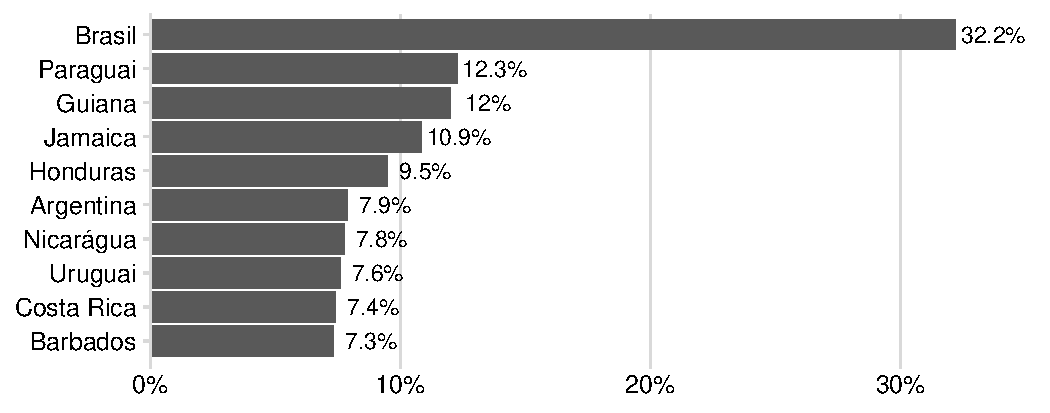
\includegraphics[width = 0.9\textwidth, scale=1]{spread_AL.pdf}
        \legend{Fonte: indicador ``FR.INR.LNDP'' do World Bank. Elaboração própria}
        \label{spreadal}
    \end{figure}

    Com a bem-sucedida estabilização macroeconômica feita pelo Plano Real, esperava-se que esse nível finalmente começasse a convergir para os padrões internacionais mas, embora ele tenha de fato se reduzido consideravelmente, ainda continuou em um patamar relativamente elevado.

    Desde então, uma das principais razões que se atribui a isso é a política monetária, conduzida sob o Regime de Metas de Inflação (RMI) desde 1999, de manter a níveis altos a taxa básica de juros com o objetivo de controlar a inflação, porque ela indexa parte dos títulos da dívida pública brasileira, o que torna a compra de títulos públicos mais atraente que o crédito, uma aplicação naturalmente mais arriscada e menos líquida \cite[p.~7]{manhica12}.
    
    Mais recentemente, o debate foi reanimado devido à persistente queda da taxa Selic, trazendo consigo a expectativa de queda também do spread. Embora essa queda tenha mesmo se efetivado, seu ritmo foi tido como insatisfatório pelas autoridades \cite{valor1}. Há um elenco de fatores que podem ajudar a explicar isso, de variáveis micro, como a concorrência, assimetrias de informação sobre os tomadores de crédito e capacidade de recuperação de garantias\footnote{Ver \cite[p.~13]{reb2018}.}, a macroeconômicas, como a inadimplência e concentração bancária\footnote{Ver \cite{valor2}}.
    
    Em um cenário de incerteza macroeconômica, é interessante que se investigue os determinantes macroeconômicos do spread bancário, a fim de, com um melhor entendimento do caso brasileiro, contribuir para a efetividade das políticas de redução do spread, o que se apresenta ainda mais importante na atual situação de estagnação econômica, já que um spread mais baixo poderia ajudar na retomada, ao facilitar o acesso ao crédito dos agentes econômicos e, portanto, a realização de investimentos \cite[p.~8]{manhica12} além de, de modo geral, significar um sistema financeiro mais desenvolvido, mais eficiente em seu papel da intermediação financeira.

\section{Visualização e análise descritiva das variáveis}

    Neste capítulo serão apresentadas as relações teóricas entre a variável dependente e as variáveis independentes incluídas no modelo, assim como a evolução histórica das séries, que cobrem o período de março de 2011 até outubro de 2019.

    Começaremos com o spread bancário. Trata-se, mais especificamente, da série 20786 do Sistema Gerenciador de Séries Temporais (SGS) do Banco Central do Brasil, intitulada "Spread médio das operações de crédito com recursos livres - Total", sendo a diferença, em pontos percentuais, entre a taxa média de empréstimo e de captação no mês. Por total, entende-se que ela aglutina operações de pessoas físicas e jurídicas, e por recursos livres, que exclui operações envolvendo taxas regulamentadas, lastreadas em recursos governamentais e afins.

    \begin{figure}[h]
        \centering
        \caption{Spread médio das operações de crédito com recursos livres - Total}
        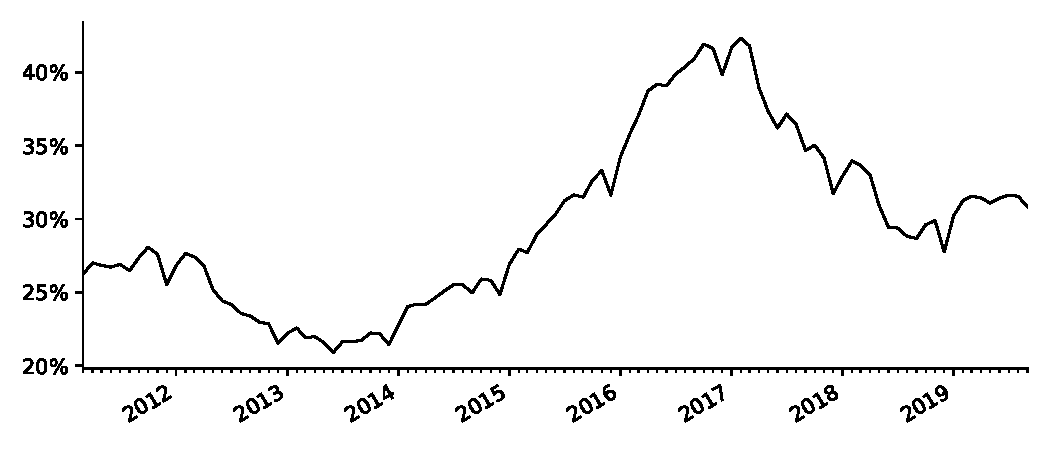
\includegraphics[width=\textwidth, scale=0.75]{spread.pdf}
        \legend{Fonte: série 20786 do SGS\@. Elaboração própria}
        \label{spread}
    \end{figure}

    Na literatura, é o que se conhece por spread \textit{ex-ante}, porque é calculado com base não no resultado financeiro efetivo dos bancos, mas nas taxas que eles estabelecem, ou seja, no que eles esperam ganhar. Por isso, essa decisão é consideravelmente influenciada por suas expectativas em relação à economia, sendo portanto mais sensível a mudanças macroeconômicas e ao risco percebido \cite[p.~226]{leal07}. Em contraste, o spread \textit{ex-post} é calculado com base na receita e despesa efetiva advinda da atividade de intermediação financeira \cite[p.~2]{almeida15}. 
    
    Na \autoref{spread}, podemos ver o aumento do spread que ocorreu a partir de 2014, após uma queda que se iniciou por volta de 2012 e que corresponde às políticas do primeiro governo de Dilma Rousseff com o intuito de reduzir o spread via aumento do portfólio de crédito dos bancos públicos, forçando uma queda pela competição das taxas de juros de empréstimos \cite[p.~1]{almeida15}. Com a deterioração das condições macroeconômicas a partir de 2014, o spread entra em escalada, seguida por um declínio iniciado em 2017 por conta da, entre outras coisas, queda persistente da taxa Selic a partir de então.

    Este movimento da taxa Selic pode ser visto na \autoref{selic}. 2. A contraposição das duas séries sugere de imediato que elas são positivamente correlacionadas. De fato, é isso o que naturalmente se argumenta, porque uma taxa básica de juros mais elevada implica maior custo de oportunidade para a atividade de crédito, uma vez que aumenta a rentabilidade dos títulos públicos, tornando mais atrativa uma aplicação que já tem a vantagem de ser mais líquida e menos arriscada \cite[p.~372]{oliveira2007}. Por esta razão, é esperado um coeficiente positivo para a taxa básica de juros, pelo efeito custo de oportunidade. Na literatura empírica, não há divergências para essa estimativa, tendo a maior parte dos estudos encontrado a relação esperada \cite[p.~233-234]{leal07}.

    \begin{figure}[h]
        \centering
        \caption{Taxa de juros - Selic acumulada no mês anualizada}
        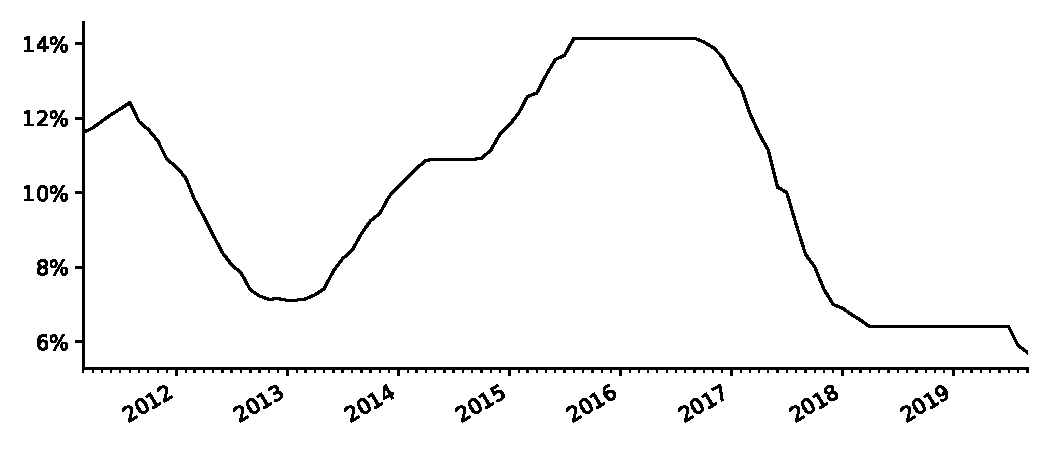
\includegraphics[width = \textwidth, scale=0.75]{selic.pdf}
        \legend{Fonte: série 4189 do SGS\@. Elaboração própria}
        \label{selic}
    \end{figure}

    Um padrão parecido pode ser observado na série da Inadimplência, na \autoref{inad}, que passou a cair consideravelmente em 2012 para depois aumentar a partir de 2014 e 2015, com o advento da crise econômica. Não é surpreendente que haja aqui uma correlação com a Selic, visto que um aumento da taxa básica de juros eleva o custo de captação, que é então repassado para o juros final, prejudicando a capacidade de pagamento \cite[p.~390]{oliveira2007}. A inclusão desta variável, portanto, serve para capturar o efeito do risco de crédito sobre o spread, \textit{ceteris paribus}.

    \begin{figure}[t]
        \centering
        \caption{Inadimplência da carteira de crédito - Total}
        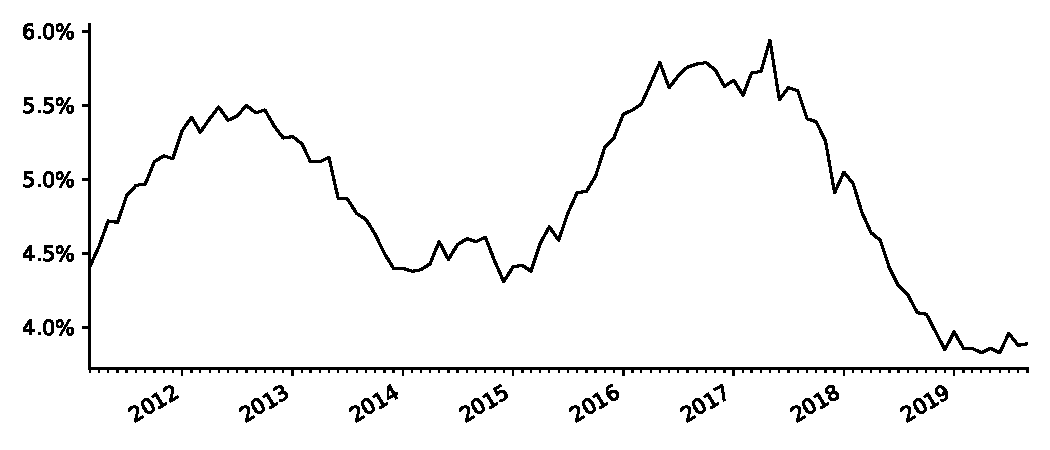
\includegraphics[width = \textwidth, scale=0.75]{inad.pdf}
        \legend{Fonte: série 21085 do SGS\@. Elaboração própria}
        \label{inad}
    \end{figure}

    A série de inflação escolhida foi a taxa anualizada do Índice Geral de Preços (IGP-DI), por ter apresentado resultados mais consistentes que o IPCA \cite[p.~66]{rocha09} e por ser mais abrangente \cite[p.~21]{afanasieff02}, tendo como desvantagem maior volatilidade e por não ser a oficialmente utilizada pelo regime de metas de inflação \cite[23]{chaim}. Ela pode ser visualizada na \autoref{igp}.
    
\begin{figure}[h]
  \centering
    \caption{Índice Geral de Preços (IGP-DI)}
      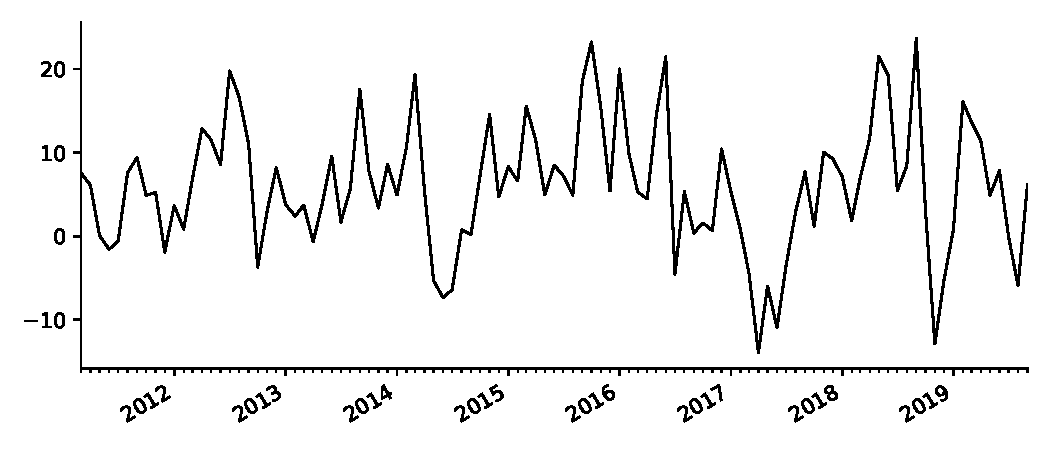
\includegraphics[width = \textwidth, scale=0.75]{igp.pdf}
      \legend{Fonte: série "PAN12\_IGPDIG12" do IPEADATA\@. Elaboração própria}
      \label{igp}
\end{figure}
    
    A inclusão dessa variável se faz necessária porque sua variação pode influenciar a taxa básica de juros e a política de juros dos bancos, portanto o spread \cite[p.~14]{bignotto06}. Além disso, pode aumentar o spread por deteriorar as expectativas dos agentes ou por fazê-los proteger sua margem nominal de intermediação financeira. O que se espera obter na estimação é um coeficiente positivo, indicando uma relação direta entre a inflação e o spread, porque em um ambiente econômico não sujeito à instabilidade dos preços os bancos não precisariam se proteger dela via spread. 
    
    Se por um lado o efeito teórico esperado é claro, o que sairá na estimação é incerto, porque na literatura varia desde insignificante, como em \textcite{oreiro}, a um sinal inesperado e significante, como em \textcite{bignotto06} e \textcite{afanasieff02}\footnote{Como possível causa, os autores indicam a apropriação de receita de senhoriagem com o spread \cite[p.~25]{afanasieff02}}.
    
    É comum na literatura incluir alguma variável para capturar a influência da atividade econômica sobre o spread. Aqui será utilizado o Índice de Atividade Econômica do Banco Central (IBC-Br), dessazonalizado e com ano-base em 2002 (\autoref{ibc}), usado para ajudar a antecipar o valor mensal do PIB como mensurado pelo IBGE.

    \begin{figure}[!hbt]
        \centering
        \caption{Índice de Atividade Econômica do Banco Central (IBC-Br) - Dessazonalizado}
        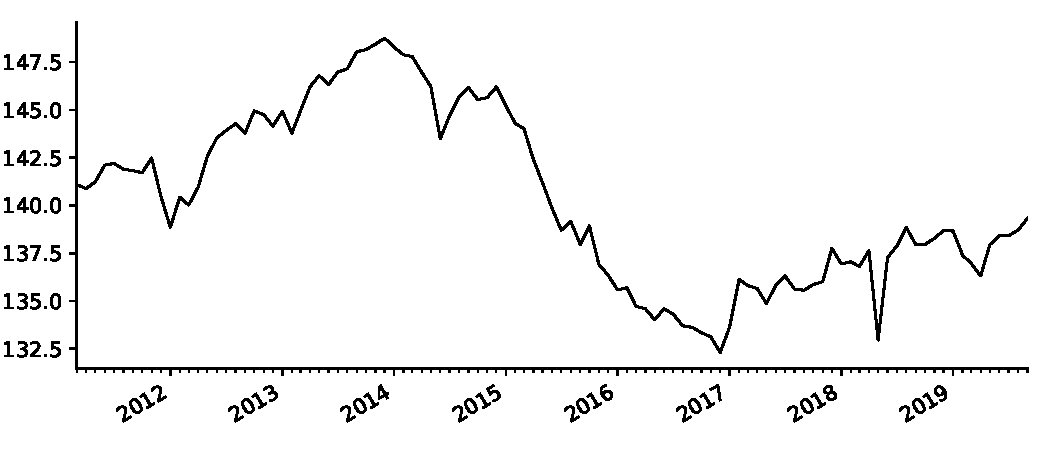
\includegraphics[width = \textwidth, scale=0.75]{ibc.pdf}
        \legend{Fonte: série SGS12\_IBCBRDESSAZ12 do IPEADATA\@. Elaboração própria}
        \label{ibc}
    \end{figure}

    Em relação ao seu efeito sobre o spread, o mais correto é considerá-lo ambíguo. Porque, por um lado, uma maior atividade econômica pode afetar positivamente o spread ao aumentar a taxa de empréstimo via aumento da demanda por crédito, o que dependerá ainda do poder de mercado dos maiores bancos \textcite[626]{oreiro}, e, por outro, pode diminuir o spread ao melhorar as expectativas dos bancos quanto ao risco de crédito \textcite[24]{chaim}. Outro possível efeito é por meio da inadimplência, ou seja, pelo efeito de uma menor (maior) atividade econômica aumentar (reduzir) a inadimplência, fazendo com que o spread aumente (diminua).

    Foi ainda considerada a inclusão do Índice de Herfindahl-Hirschmann (IHH) para capturar o efeito da concentração estrutural no Sistema Financeiro Nacional sobre o spread. Como se sabe, este é um indicador do nível de concentração econômica em um mercado, obtido ao somar o quadrado das participações de cada instituição financeira no mercado considerado, que no nosso caso é o mercado de crédito. O BCB considera um IHH entre 0 e 1000 indicativo de baixa concentração, acima de 1000 e menor que 1800, de moderada concentração e acima de 1800 de alta concentração.
    
    No entanto, o índice é divulgado somente trimestralmente e, além disso, termina no ano de 2017 como foi divulgado no Anexo Estatístico do Relatório de Estabilidade Financeira do Banco Central de abril de 2018, como pode ser visto na \autoref{ihh}. Daí se vê que a série apresenta restrições para o tamanho de amostra além de dados faltantes, o que levou à decisão de não incluí-la na estimação, apesar do interesse teórico.

    \begin{figure}[h]
        \centering
        \caption{Índice de Herfindahl-Hirschmann - IHH}
        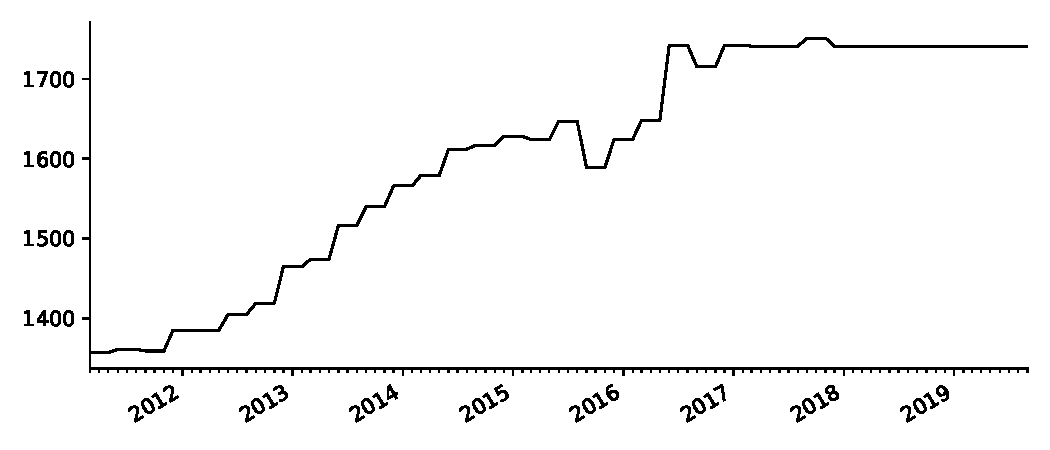
\includegraphics[width = \textwidth, scale=0.75]{ihh.pdf}
        \legend{Fonte: BCB\@. Elaboração própria}
        \label{ihh}
    \end{figure}

    Espera-se, contudo, que isso não signifique incorrer em problemas de viés de variável omitida. Apesar de não ser possível prever ao certo o sinal do coeficiente estimado para esta variável, acredita-se que o sinal esperado possa ser até mesmo não-significante, com o argumento de que seria a concorrência a variável relevante para explicar o spread, visto que há alta concentração bancária mesmo em países com um sistema financeiro eficiente e bem desenvolvido. Mas também não se descarta a possiblidade do sinal positivo, indicando influência do poder de mercado dos bancos, e até mesmo um sinal negativo, com os investimentos e ganhos de escala associados à concentração aumentando a eficiência da atividade de intermediação, o que puxa o spread para baixo \cite{reb2017}. 

    Da \autoref{ihh} pode-se concluir que houve um aumento na concentração bancária durante o período. Em contraposição a isso, no \textcite[11]{reb2017} é apontando um aumento da concorrência bancária no mesmo período, o que explicita que nem sempre essas variáveis andam juntas.

    Por fim, a \autoref{tab1} sumariza o que foi aqui discutido, listando cada variável e seus sinais esperados, além de algumas estatísticas descritivas.

    \begin{table}[h]
        \IBGEtab{\caption{Tabela de estatísticas descritivas}\label{tab1}}
        {%
            \begin{tabular}
                {@{\extracolsep{5pt}}lccccc}
                \midrule
                Variável              & \multicolumn{1}{c}{Média} & \multicolumn{1}{c}{Desvio Padrão} & \multicolumn{1}{c}{Mín.} & \multicolumn{1}{c}{Máx.} & \multicolumn{1}{c}{Sinal esperado} \\
                \midrule
                Spread                & 29,33                     & 6,51                              & 20,89                    & 42,34                    &  \\
                Selic                 & 10,96                     & 2,37                              & 7,00                     & 14,15                    & + \\
                Inadimplência         & 5,09                      & 0,47                              & 4,31                     & 5,94                     & + \\
                IGP-DI                & 5,74                      & 7,33                              & $-$13,93                 & 23,26                    & + \\
                Atividade Econômica   & $-$2,28                   & 4,86                              & $-$13,39                 & 9,70                     & +/- \\
                IHH                   & 1.566,30                  & 133,69                            & 1.357                    & 1.751                    & + \\
                \midrule
            \end{tabular}
        }
        {\fonte{Elaboração própria.}\nota{Em sinal esperado, ``+'' indica um coeficiente positivo, ``-'', um negativo.}}
    \end{table}


\section{Revisão de Literatura}
\subsection{Revisão da literatura teórica}

    Nesta seção serão apresentados dois modelos que se consagraram na literatura sobre os determinantes do spread: o modelo do banco como uma firma maximizadora de lucros de \textcite{klein} e o modelo do banco como intermediador financeiro de \textcite{hoesaunders}. O intuito é ajudar a entender quais e como as variáveis são relevantes para explicar o spread bancário.

\subsubsection{O Banco como firma}

    Neste modelo, o banco é visto como uma firma que produz serviços voltados para intermediar a oferta e demanda de crédito, receber depósitos (D) e fazer empréstimos (L), a uma taxa de juros determinada em um mercado monopolístico ou semi-monopolístico, ou seja, em que é possível fixar a taxa de juros acima do custo marginal de produção, o que é aqui entendido como o spread por si mesmo, como o poder de mercado deste banco. \cite{oreiro}

    O autor considera o banco como um agente neutro ao risco, por buscar maximizar somente o valor esperado do lucro, sem considerar sua variância, que se depara com uma curva de demanda por empréstimos decrescente, $ L(r_L) $, uma curva de oferta de depósitos crescente, $ D(r_D) $, e uma função custo do tipo $ C(D, L) $, em que $ r_L $ denota a taxa de juros cobrada ao emprestar, e $ r_D $ a taxa paga ao depositante. A função lucro, considerando as funções inversas, pode então ser assim expressa: 
    
    \begin{equation} \pi(D, L) = r_L(L)L + rM - r_D(D)D - C(D, L) \end{equation}
        
    em que $ r $ representa a taxa de juros do mercado interbancário, e M, o que o banco tem disponível para aplicar neste mercado, a saber, tudo o que recebe de depósito e não empresta nem vai para o compulsório (uma porcentagem $\alpha$ dos depósitos), $M = (1 - \alpha)D - L$. 

    Manipulando a equação, obtemos o que representa o resultado da intermediação financeira subtraído de seus custos: 
    
    \begin{equation} \pi(L, D) = (r_L(L) - r)L + (r(1 - \alpha) - r_D(D))D - C(D, L) \end{equation}

    O próximo passo é obter a margem ótima de intermediação, isto é, a que maximiza a função lucro. Para isso, tira-se as derivadas parciais desta função em relação a L e D para se chegar às condições de primeira ordem, e, depois de algumas manipulações algébricas, chega-se às equações fundamentais do modelo:

    \begin{gather}
        \frac{1}{\epsilon^{*}_L} = \frac{r^{*}_L - (r - C^{'}_L)}{r^{*}_L} \\
        \frac{1}{\epsilon^{*}_D} = \frac{r(1-\alpha)-C^{'}_D - r^{*}_D}{r^{*}_D}
    \end{gather}

    O lado direito da equação é a versão para firma bancária do índice de Lerner\footnote{Definido como a razão $(P - C_{mg}) / P$, em que $P$ é preço e $C_{mg}$ é o custo marginal, é uma medida do poder de mercado de um agente maximizador de lucros, sendo idêntico à recíproca da elasticidade. \cite{maudos}}, sendo, por definição, em cada um dos casos, igual ao inverso da elasticidade-juros da demanda por empréstimos ($\epsilon^{*}_L$) e oferta de depósitos ($\epsilon^{*}_D$). A interpretação desse resultado é que, para maximizar seus lucros, os bancos procuram fixar a taxa de juros num nível acima de seus custos, mas não ao ponto de perderem muitos clientes para a concorrência (o que acontece mais facilmente em mercados com demanda elástica etc.).

    Segue-se imediatamente destas equações que o spread bancário será tão maior quanto menos sensíveis forem as elasticidades da demanda por empréstimo e da oferta de depósito em relação à taxa de juros. Outra implicação interessante é que se a taxa de juros $ r $ do mercado interbancário aumentar, as taxas de intermediação também irão \cite[p.~59]{freixas}.

\subsubsection{O banco como intermediador financeiro}

    Neste modelo, primeiro apresentado em \textcite{hoesaunders}, o banco é considerado como um agente que atua como intermediador entre demandantes e ofertantes de fundos. É um dos mais influentes modelos na literatura, tendo sido estendido por vários outros autores.

    Este modelo difere radicalmente do de \textcite{klein} no que tange ao tipo de mercado em que o banco atua, não mais harmônico e equilibrado, mas sujeito a incertezas. Neste cenário, o banco não é mais considerado neutro ao risco, mas avesso a ele. Isso porque se depara com duas incertezas: o risco da inadimplência e o risco da taxa de juros, que tem a ver com a possível descoordenação entre demanda por empréstimos e ofertas de depósitos, caso em que o banco terá que recorrer ao mercado interbancário. No caso de demanda excessiva de empréstimos, o banco terá que pedir emprestado e estará sujeito ao risco da taxa de juros aumentar nesse ínterim. No caso de oferta excessiva de depósitos, terá que aplicar o excesso, no que estará sujeito ao risco da taxa cair. \textcite[p.~2262]{maudos}

    Por esta razão, os bancos procuram minimizar esse risco fixando taxas de juros para os depósitos ($r_D$) e para os empréstimos ($r_L$) com a adição de uma pequena margem relativa à taxa de juros do mercado interbancário. Esta margem é o spread ($s$):

	\begin{align}
        r_D &= r - a \\
        r_L &= r + b \\
        s &= r_L - r_D = a + b
	\end{align}

    Para uma derivação das equações do modelo, até a equação do spread ótimo, ver \textcite[p.~2262]{maudos} ou \textcite[p.~584]{hoesaunders}. Para propósitos da revisão, iremos omiti-la, considerando somente suas implicações no que concerne aos determinantes do spread. São eles:

	\begin{enumerate}
		\item Estrutura competitiva do mercado: o que se relaciona com as elasticidades-juros da demanda por empréstimo e da oferta de depósitos, como em \textcite{klein}.
		\item Aversão ao risco: quanto mais avessos, maior o spread.
		\item Volatilidade da taxa de juros do mercado interbancário: quanto mais instável a taxa de juros, maior o risco, e portanto maior o spread.
		\item Inadimplência: quanto maior o risco de inadimplência, mais o bancos terão que se proteger via spread.
		\item Covariância entre risco da taxa de juros e de inadimplência: captura a influência da instabilidade macroeconômica na insolvência das famílias.
		\item Tamanho médio das operações de crédito e de depósito: uma operação de tamanho maior que o médio significa maior perda potencial, da qual se protege com um spread maior.
	\end{enumerate}

    Esse modelo teórico é a base sob a qual se sustenta a abordagem empírica dos mesmos autores: a estimação do spread em dois estágios. Primeiro, estima-se o spread "puro", ao regredir o spread sobre as variáveis não incluídas no modelo teórico como controle, comumente variáveis microeconômicas e características dos bancos, para então regredir os resíduos dessa regressão contra as variáveis do modelo teórico \textcite{maudos}. Uma das vantagens dessa abordagem está em sua flexibilidade, permitindo a inclusão de variáveis sem grandes problemas \textcite[p.~2]{almeida15}.

\subsection{Revisão da literatura empírica}

    Esta seção procura revisar os estudos empíricos sobre os determinantes do spread bancário calculado com base nas taxas de juros prefixadas cobradas nas modalidades de crédito com recursos livres e na taxa de captação de CDB de trinta dias.

    A estabilidade macroeconômica e as políticas governamentais que se seguiram ao Plano Real possibilitaram uma queda significativa do spread bancário, porém somente até um nível consideravelmente alto para os padrões internacionais. Somando-se a isso a reestruturação bancária observada no período, \textcite{afanasieff02} notam que além da grande variação temporal do spread, há também uma grande variação interbancária. É nesse sentido que os autores justificam o emprego de técnicas de dados em painel, com o objetivo de capturar essas características do mercado bancário brasileiro para a decomposição dos principais determinantes do spread em variáveis micro e macroeconômicas.

    Para isso, os autores aplicam a metodologia de dois passos de \textcite{hoesaunders}, usando dados mensais de 142 bancos para o período de fevereiro de 1997 a novembro de 2000, formando um painel com 5578 observações. Para a estimação do spread puro, usam como regressores o intercepto, um vetor temporal (tendência determinística) e um de características bancárias como controle\footnote{Dentre elas, número de agências, custos operacionais, a taxa de depósitos à vista e a prazo em relação ao ativo total, a liquidez, o pagamento de juros implícitos, a alavancagem, uma variável dummy para banco estrangeiro, a receita de serviços sobre a receita operacional total e o patrimônio líquido}. Uma vez estimado o spread puro, dado nesse caso pelos coeficientes do vetor temporal e do intercepto, ele é então regredido sobre as variáveis macroeconômicas: a taxa de inflação, o compulsório, a taxa Selic, o crescimento do PIB, a taxação financeira e uma proxy para prêmio de risco.

    No primeiro estágio, foi encontrado que o custo operacional, a taxa de depósitos à vista em relação ao ativo total e a de receita de serviços em relação à receita operacional afetam positivamente o spread, e que os bancos estrangeiros estão em média associados a um spread menor. Os autores, ao contraporem o spread puro estimado com o observado, apontam ainda que os fatores microeconômicos não parecem ser os principais determinantes do spread.
    
    Pelos resultados do segundo estágio, há uma relação direta e significativa entre spread e taxa básica de juros, risco, taxação financeira e crescimento do PIB, e contrária no caso da inflação. O efeito estimado do compulsório não foi significativo.

    Seguindo linha metodológica parecida, \textcite{bignotto06} também se utilizam do modelo teórico de \textcite{hoesaunders} para analisar a influência dos custos de intermediação e dos fatores de risco de crédito e de juros sobre o spread. Para a estimação, fez-se uso de dados de 87 bancos brasileiros ao longo do 1º trimestre de 2001 até o 1º trimestre de 2004, formando uma base de dados em painel desbalanceado com 1131 observações.
    
    Foram usados como regressores o custo administrativo, uma proxy para o risco de crédito e de juros, o market-share, o risco de liquidez, a taxa de receitas de serviços sobre o ativo total e a da despesa tributária sobre o ativo total, o compulsório, a Selic, a inflação e o ativo total de cada banco corrigido pela inflação, além de uma variável não-observável de aversão ao risco como controle. 
    
    O modelo que os autores julgam mais eficiente revela uma relação direta entre o spread e os custos administrativos, o risco de crédito e de juros, o compulsório, a Selic, e o ativo total, todos com o sinal esperado. Algumas variáveis de controle apresentaram coeficientes inesperados, como no caso da liquidez, da receita de serviços e do market share. Já a variável relativa à carga tributária não se mostrou significativa.

    Complementando os importantes estudos feitos pelo Banco Central do Brasil à época, que consistiam na decomposição contábil do spread, \textcite{nakane02} buscaram investigar a sensibilidade do spread a variações nas variáveis que o compõem, isto é, investigar o assunto por um abordagem econométrica. Para isso, os autores utilizaram a seguinte equação:

    $$\ln spread = \beta_0Tend + \beta_1\ln selic_t + \beta_2\ln adm_t + \beta_3\ln risk_t + \beta_4\ln imp_t + \beta_4\ln comp_t$$

    Em que $ selic $ é a taxa básica de juros, $ adm $ é a razão das despesas administrativas sobre o volume de crédito, $ risk $ é uma proxy de risco global\footnote{"[É] o spread do rendimento do C-Bond sobre o rendimento do título do Tesouro americano com mesma maturidade." \cite[p.~10]{nakane02}} que busca capturar expectativas, $ imp $ é uma medida da incidência de tributos indiretos sobre o spread, $ comp $ é a taxa de compulsório sobre depósitos à vista exigida pelo Bacen, $ Tend $ é uma medida de tendência determinista incluída com o intuito de controlar para variáveis que não foram incluídas na equação, como a taxa de inflação, o nível de atividade econômica etc., e $ \ln $ é o logaritmo natural. Para mais detalhes, ver \textcite[10]{nakane02}.

    Para a estimação da equação de longo prazo, foram usados dados mensais do período de agosto de 1994 a setembro de 2001 em um modelo de vetores autorregressivos (VAR) que, uma vez tratado estatisticamente, revelou que a taxa Selic, as despesas administrativas, o risco e os impostos indiretos afetam positiva e significativamente o spread. Já o compulsório não se mostrou significativo e foi retirado do modelo.

    Em seguida, os autores decompuseram o spread do período com base nessa estimação. O resultado indica que todas as variáveis são bem relevantes na composição do spread no período, em especial a variável de risco, relevância esta que foi aumentando com o passar dos anos e que é análoga à considerável participação da inadimplência na decomposição contábil do spread. Os custos administrativos e a Selic vêm em seguida em importância, ambas com tendências sutilmente declinantes. E, por fim, a importância relativa dos impostos indiretos é a menos sobressalente, mas aumentou com os anos. 

    Um artigo que segue um caminho semelhante em termos de modelagem é o de \textcite{oreiro}, já que para a estimação dos determinantes também se utilizou um modelo VAR\@. Este estudo, porém, se distingue por dar foco aos efeitos das variáveis macroeconômicas sobre o spread, cobrindo o período de janeiro de 1995 a dezembro de 2003. 
    
    São usados como regressores séries de frequência mensal como o nível da taxa básica de juros (Selic) e sua volatilidade (como proxy para o risco de juros), o nível de atividade econômica, o recolhimento compulsório sobre depósitos à vista e a inflação.

    Para interpretar os coeficientes estimados, os autores se utilizaram da função de impulso-resposta, em que se procurou observar o efeito de longo prazo que um choque exógeno de um desvio-padrão em uma variável independente tem sobre a variável dependente. A decomposição da variância também foi utilizada, com objetivo similar. Em ambos os casos, busca-se enxergar o efeito estimado do choque ao longo de 12 meses.

    Os resultados mostram que um choque exógeno no nível e volatilidade da taxa de juros tem um efeito positivo e persistente sobre o spread, como esperado. Um choque na proxy para o nível de atividade econômica mostrou ter um impacto positivo, o que os autores interpretaram como um possível efeito do poder de mercado dos bancos prevalecendo sobre o efeito inadimplência. O efeito de um choque na inflação se mostrou insignificante estatisticamente. Eles concluem dizendo que um ambiente macroeconômico estável é uma condição indispensável para reduzir o spread.

    O trabalho mais recente de \textcite{chaim} é talvez o que mais se assemelha ao presente trabalho. Isso porque estuda os determinantes do spread ex-ante no período de janeiro de 2004 a dezebro de 2012, quando termina a série como calculada pela antiga metodologia do Banco Central, sob um ponto de vista econométrico, usando o ferramental teórico dos vetores autorregressivos.

    Nele estão inclusas variáveis como a Selic (nível e volatilidade\footnote{Cuja proxy é o \textit{spread over treasury}, a diferença entre as taxas que remuneram os títulos da dívida pública brasileira e estado-unidense, com maturidade de seis meses}), dois indicadores para a inflação, o IPCA e o IGP, quatro indicadores para a atividade econômica\footcite[20]{chaim} e a taxa de câmbio. Foram estimados oito modelos vetoriais de correção de erros distintos, um para cada combinação das diferentes medidas de variável de inflação e atividade econômica, a fim de testar a robusteza dos resultados, isto é, se os sinais são invariantes às medidas. 

    Nas funções de impulso-resposta, foi consistentemente encontrado que um impulso no nível e na volatilidade da Selic aumenta persistentemente o spread. Já um impulso na taxa de câmbio ocasiona um aumento temporário no spread, talvez porque os bancos tenham que reestruturar seu portfólio de crédito, o autor menciona. Um impulso na inflação é seguido de um choque positivo, um sinal de que os bancos tentar sua margem de intermediação quando a taxa de juros real cai. Por fim, foi encontrado que um choque na atividade econômica impacta negativamente o spread a princípio, possivelmente por indicar menor risco de crédito, mas depois passa a impactar positivamente, talvez pelo aumento na demanda por crédito. Para esta variável, no entanto, os resultados não foram tão consistentes através dos modelos, exceto para as medidas de hiato do produto, cuja resposta ao impulso se mostrou majoritariamente positiva \cite[32-38]{chaim}.

\section{Referencial Metodológico}

    Neste capítulo serão brevemente apresentadas as metodologias utilizadas para a modelagem e tratamento de séries temporais.

    Todo estudo do tipo requer primeiro que conheçamos a ordem de integração das séries, isto é, se é estacionária (caso em que é integrada de ordem 0) ou, caso contrário, quantas $d$ vezes é preciso diferenciá-la para que se torne estacionária (caso em que será integrada de ordem $d$), o que é mais formalmente feito com um teste de raiz unitária.

    Uma vez que se saiba quais são as séries não-estacionárias, é prudente investigar se alguma combinação linear delas é estacionária, ou seja, se há co-integração.

    Os resultados destes dois testes influenciam enormemente na decisão de como modelar o relacionamento entre as séries. 

    \subsection{Teste de raiz unitária}

    Na análise de séries temporais, é comum nos assegurarmos de que elas sigam um processo estocástico cujas variáveis aleatórias tenham média e variância constante e finita e função de autocovariância que dependa somente da defasagem no tempo e não do tempo em si \cite[p.~734]{gujarati}, isto é, que sejam estacionárias no sentido amplo. Mais formalmente, um processo aleatório formado por variáveis aleatórias discretas $Y_t$ será estacionário se, dado um processo estocástico autorregressivo de ordem 1 do tipo:

    \begin{equation}\label{processo_estocastico} Y_t = \rho Y_{t-1} + u_t \end{equation}

    Onde $ u_t \stackrel{iid}{\sim} \text{N}(0,\text{ }\sigma^2) $. Sabe-se que ele será estacionário se $ \lvert \rho \rvert < 1 $, e não-estacionário se $ \lvert \rho \rvert = 1 $, o que é conhecido como passeio aleatório\footnote{Ao resolver recursivamente para o caso quando $ \lvert \rho \rvert = 1 $, $ Y_t = Y_{t-1} + u_t = Y_0 + \sum u_t $, percebe-se a importante característica de memória infinita do processo, de que ele nunca se "esquece" do choque. \cite[p.~736]{gujarati}}.

    O objetivo do teste de raiz unitária é inferir o valor de $ \rho $ com base nas realizações particulares do processo estocástico. Isto é útil porque assim podemos saber se teremos que trabalhar com as variáveis em primeira diferença (para evitar regressões espúrias) ou testar se elas co-integram.
    
    Para isto, o teste \textit{Augmented Dickey-Fuller} modifica a \autoref{processo_estocastico} como segue:

    \begin{align}
        \label{adf}
        Y_t - Y_{t-1} &= \rho Y_{t-1} - Y_{t-1} + \sum_{i = 1}^{p-1}\delta \Delta Y_{t-i} + u_t \nonumber \\
        \Delta Y_t &= \gamma Y_{t-1} + \sum_{i = 1}^{p-1}\delta \Delta Y_{t-i} + u_t
    \end{align}

    Onde $ \gamma = (\rho - 1) $. Para logo depois estimar esta equação por Mínimos Quadrados Ordinários (MQO).
   
    O valor estimado de $ \gamma $ serve então para testar a hipótese de raiz unitária $ \gamma = 0 $, que equivale a $ \rho = 1 $, contra a hipótese alternativa unilateral $ \gamma < 0 $, que equivale a $ \rho < 1 $. Calcula-se então o valor t estimado, isto é, $ \hat{\gamma} / \text{EP}(\hat{\gamma}) $, com o porém de que sob a hipótese nula $ \gamma = 0 $, essa estatística não segue mais a distribuição t, mas a distribuição $ \tau $. Isso se dá em razão do teste t ser enviesado no caso de um passeio aleatório \cite[p.~748-749]{gujarati}.

    Importante pontuar que a estatística $ \tau $ é sensível à forma funcional da equação \eqref{processo_estocastico}, isso quer dizer que os valores críticos do teste mudarão se adicionarmos um termo de deslocamento $ \delta $ em \eqref{processo_estocastico}, denotada como $ \tau_{\mu} $ ou um termo de tendência determinística, $ \beta t $, $ \tau_{\tau} $.
   
    O termo adicional $ \sum_{i = 1}^{p-1}\delta \Delta Y_{t-i} $ em \eqref{adf} serve para generalizar o teste para processos autorregressivos de ordem $ p $, de forma a preservar a condição de ruído branco em $ u_t $ ao controlar pela possível autocorrelação serial \cite[p.~40]{gustavo}.

    Serão ainda utilizados os testes de Phillips-Perron e de Kwiatkowski-Phillips-Schmidt-Shin, apesar de não serem expostas aqui em detalhes. Para isso, ver \textcite{pp} e \textcite{kpss}.

    Uma série é dita integrada de ordem 0 quando for diagnosticada como estacionária, $ Y_t \sim I(0) $, e integrada de ordem 1, $ Y_t \sim I(1) $, quando não é possível rejeitar a hipótese nula de raiz unitária, implicando que sua primeira diferença é estacionária.

    \subsection{Teste de Co-integração}

    Quando duas ou mais séries são integradas da mesma ordem, mas uma combinação linear delas for integrada de uma ordem menor, dizemos que elas co-integram. O caso comum é quando as séries são não-estacionárias, mas uma combinação linear delas é estacionária.
    
    Formalmente, as séries $ \mathbf{Y_t} $ são co-integradas de ardem $ d, b $ se todas forem integradas de ordem $ d $ e se existe uma combinação linear $ \mathbf{Z_t} = \pmb{\beta}'\mathbf{Y_t} $ tal que $ \mathbf{Z_t} \sim I(d - b), b > 0 $ \cite[p.~245]{lutkepool}, onde $ \pmb{\beta} $ é o vetor cointegrante.

    O teste de Engle-Granger procura testar essa condição em duas etapas. Por exemplo, em um contexto bi-variado, em que $ Y_t $ é explicada por $ X_t $, primeiro estima-se a seguinte equação por MQO:

    \begin{equation}
        Y_t = \beta_0 + \beta_1 X_t + u_t \label{engle-granger}
    \end{equation}

    Para na segunda etapa, aplicar o teste ADF nos resíduos desta regressão, ou seja, na equação $ \Delta \hat{u}_t = \gamma \hat{u}_{t-1} + \epsilon_{t} $. Se eles forem estacionários, então pode-se concluir que as séries são co-integradas.

    Vale ressaltar que, como explicado por \textcite[p.~756]{gujarati}, os valores críticos com os quais se deve comparar a estatística de teste calculada são diferentes dos do teste de raiz unitária, porque os resíduos a serem testados foram obtidos com base no $ \beta $ estimado.

    Uma vez que é possível haver mais de uma relação de co-integração, este teste não é muito apropriado para achá-las visto que se baseia nos resultados de uma única regressão. Além disso, ele depende da especificação da equação, de qual variável é endógena e quais são exógenas. Por isso, é apropriado que se investigue a co-integração no contexto multivariado, o que será feito pelo teste de Johansen, como veremos.

    \subsection{Modelo uni-equacional de correção de erros}

    Quando duas ou mais variáveis co-integram, a interpretação econômica é de que, apesar da tendência estocástica torná-las imprevisíveis individualmente, há um mecanismo de equilíbrio de longo prazo que as impede de se afastarem uma da outra, um mecanismo de correção de erros. No curto prazo, pode haver desequilíbrio, mas ele não sai do controle (não tem uma variância explosiva), retornando sempre à uma média constante, ao contrário de um passeio aleatório \textcite[757-758]{gujarati}.

    Uma vez identificada uma relação de co-integração, é interessante que se estime a sua representação como um mecanismo de correção de erro. Nesta representação, podemos observar o quanto a variação da variável dependente é sensível ao desvio em relação ao equilíbrio e às variações de suas variáveis explicativas. Matematicamente, 

    \begin{equation}
        \Delta Y_t = \alpha_1 (Y_t - \beta_0 - \beta_1 X_t) + \alpha_2 \Delta X_t + u_t \label{ecm}
    \end{equation}

    Onde $ u_t $ é um termo de ruído branco. 
    
    Como explicado em \textcite{coint1}, o coeficiente $ \lvert \alpha \rvert $ indica o quão rapidamente a variável dependente retorna ao equilíbrio, sendo ele normalmente negativo: quando o desvio é positivo, tudo o mais constante, $ Y_t $ será corrigido para baixo, quando positivo, para cima. Ou seja, este modelo é útil para capturar a sensibilidade aos desvios da relação de longo prazo, enquanto os coeficientes das variáveis defasadas, os efeitos das mudanças de curto prazo.
    
    Neste trabalho, serão estimados tanto um modelo univariado quanto um multivariado, cuja metodologia será explorada a seguir.

    \subsection{Vetores autorregressivos (VAR)}

    Segundo \textcite[51-52]{gustavo}, a principal característica de um modelo VAR é o tratamento simétrico das variáveis incluídas no modelo, isto é, não é preciso especificar previamente quais variáveis são exógenas e endógenas, o modelo estrutural que espelha o relacionamento real das variáveis. Por isso, ele está sujeito a poucas restrições teóricas. É somente necessário especificar quais variáveis interagem dentro do sistema e o número de defasagens que melhor capturam esta interação.
    
    São muito úteis para visualizar como uma variável responde a um choque em outra variável, por causa das funções de impulso-resposta. 

    Seguindo a notação de \textcite[p.~13]{lutkepool}, um modelo de vetores autorregressivos de ordem p, VAR(p), com K variáveis, possui a seguinte forma:

    \begin{equation}
        \label{VAR}
        y_t = v + A_1 y_{t-1} + \cdots + A_p y_{t-p} + u_t,\text{\ \ } t = 0, \pm 1, \pm 2, \ldots
    \end{equation}

    Onde $ y_t = (y_{1t}, \ldots, y_{Kt})^{'} $ é um vetor de variáveis aleatórias, $ v  = (v_{1}, \ldots, v_{K})^{'}  $, um vetor para o intercepto, $ u = (u_{1}, \ldots, u_{K})^{'} $, um vetor de ruído branco gaussiano\footnote{Logo, $ \mathbf{E}(u_t) = 0 $ e $ \mathbf{E}(u_t u^{'}_t) = \Sigma_{u} $, onde $ \mathbf{E}(u_tu^{'}_s) = 0 $ para $ t \neq s $ e $ \mathbf{E}(u_t u^{'}_t) = \Sigma_u, \forall t $.} e $ A_i $ são matrizes $ (K \times K) $ de coeficientes.

    Desta equação pode-se perceber que os valores presentes das variáveis são explicados pelas $ p $ defasagens de todas as outras variáveis no sistema.

    Dado um AR(1) que começa em $ t = 1 $, resolvendo recursivamente o sistema, chegamos a:

    \begin{align}
        \label{VAR1}
        \begin{aligned}
        y_1 &= v + A_1 y_0 + u_1 \\
        y_2 &= v + A_1 y_1 + u_2 = v + A_1(v + A_1y_0 + u_1) + u_2 \\
            &= (I_K + A_1)v + A^{2}_1 y_0 + A_1 u_t + u_t \\
        y_t &= (I_K + A_1 + \dots + A^{t-1}_1)v + A^{t}_1 y_0 + \sum^{t-1}_{i=0} A^{i}_1 u_t
        \end{aligned}
    \end{align}

    Se todos os autovalores em módulo da matriz $ A_1 $ são menores que 1, o que é equivalente a testar se $ det(I_{K} - A_1z) \neq 0 $ para $ \lvert z \rvert \leq 1 $, o VAR é dito estável e converge assintoticamente para

    \begin{equation}
        \label{ma}
        \begin{aligned}
        y_t &= (I_K - A_1)^{-1} v + \sum^{\infty}_{i=0} A^{i}_1 u_{t-1} \\
        y_t &= \mu + \sum^{\infty}_{i=0} A^{i}_1 u_{t-1}
        \end{aligned}
    \end{equation}

    O que é também conhecido como a representação em média móvel do modelo VAR\@ \cite[18]{lutkepool}. Dela podemos ver que a distribuição de probabilidades de $ y_t $ é unicamente determinada pela distribuição do termo de erro $ u_t $, que se assume ser gaussiano. Esse resultado pode ser generalizado para AR(p), dado que qualquer processo AR(p) pode ser representado como um processo AR(1) \cite[p.~15]{lutkepool}. Da equação \eqref{ma} a média e auto-covariâncias de $ y_t $ podem ser derivadas: 

    \begin{align*}
        \label{momentos}
        \mathbf{E}(y_t) &= \mu, \forall t \\
        \Gamma_y (h) &= \mathbf{E}(y_t - \mu)(y_{t-h} - \mu)^{'} = \sum_{i=0}^{\infty} A_1^{h+i} \Sigma_u A_1^{i}^{'} \\
    \end{align*}

    Do que se conclui que um modelo AR(p) estável é estacionário no sentido amplo \cite[p.~15-16]{lutkepool}

    \subsection{Função de Impulso-resposta}

    A função de impulso-resposta serve para visualizar o efeito provocado em um sistema dinâmico por um choque exógeno em uma variável.

    Para vermos o que ocorre matematicamente, seguimos a exposição de \textcite[p.~51-53]{lutkepool} e supomos um AR(1) com $ v = 0 $, ou seja, $ y_t = A_1 y_{t-1} + u_t $:

    \begin{equation*}
        \begin{bmatrix}
            y_{1,t} \\
            y_{2,t} \\
            y_{3,t}
        \end{bmatrix} =
        A_1
        \begin{bmatrix}
            y_{1,t-1} \\
            y_{2,t-1} \\
            y_{3,t-1}
        \end{bmatrix} +
        \begin{bmatrix}
            u_{1,t} \\
            u_{2,t} \\
            u_{3,t}
        \end{bmatrix}
    \end{equation*}

    Se assumirmos que no período $ t = 0 $ há um choque exógeno em $ y_1 $, tal que

    \begin{equation*}
        \begin{bmatrix}
            y_{1,0} \\
            y_{2,0} \\
            y_{3,0}
        \end{bmatrix} =
        \begin{bmatrix}
            u_{1,0} \\
            u_{2,0} \\
            u_{3,0}
        \end{bmatrix} =
        \begin{bmatrix}
            1 \\
            0 \\
            0
        \end{bmatrix}
    \end{equation*}

    Teremos, em $ t $ períodos a frente, que

    \begin{equation*}
        \begin{bmatrix}
            y_{1,t} \\
            y_{2,t} \\
            y_{3,t}
        \end{bmatrix} =
        A_1^{t}
        \begin{bmatrix}
            1 \\
            0 \\
            0
        \end{bmatrix}
    \end{equation*}

    Do que se conclui que a resposta do sistema a um impulso na variável $ y_1 $ é simplesmente a primeira coluna da matriz $ A_1^{t} $, ou, mais geralmente, a resposta a um impulso na variável $ y_k $, após $ t $ períodos, é a coluna $ k $ da matriz $ A_1^{t} $, que, deve-se observar, vai se aproximando de zero quando $ i $ tende ao infinito se o VAR(1) é estável, ou seja, a resposta do sistema vai se dissipando com o tempo. Quando ele não é estável, isso não é necessariamente verdade, como no caso do modelo vetorial de correção de erros.

   Um problema dessa interpretação é a possibilidade de duas variáveis distintas serem significativamente correlacionadas, caso em que se recomenda a visualização da função de resposta ao impulso ortogonal, pois, neste caso, um choque não pode ser assumido independente um do outro, sendo provável que seja acompanhado de um choque na variável com que está correlacionado no período $ 0 $. Para resolver isso, faz-se uso da decomposição de Cholesky, que decompõe a matriz de co-variância dos resíduos $ \Sigma_u $ em uma matriz triangular inferior $ P $, tal que $ \Sigma_u = PP^{'} $, de forma a obter resíduos não correlacionados entre si (ortogonais).

   Um dos problemas da função de impulso resposta é sua sensibilidade à ordenação das variáveis.

    \subsection{Modelo vetorial de correção de erros (VECM)}

    Como há a possiblidade de múltiplas relações de equilíbrios entre as variáveis sob análise, gostaríamos de identificá-las, o que será feito com o teste de Johansen, para depois modelar suas evoluções temporais como um mecanismo de correção de erros multivariado.

    A diferença em relação ao caso univariado é que agora temos mais de uma equação. Por exemplo, dadas duas variáveis $ I(1) $, $ y_1 $ e $ y_2 $, teremos que:

    \begin{equation}
        \begin{aligned}
            \label{ecm_vec}
            \Delta y_{1t} = \alpha_1 (y_{1,t-1} - \beta_1 y_{2, t-1}) + \gamma_{11,1} \Delta y_{1,t-1} + \gamma_{12,1} \Delta y_{2,t-1} + u_{1t} \\
            \Delta y_{2t} = \alpha_2 (y_{1,t-1} - \beta_1 y_{2, t-1}) + \gamma_{21,1} \Delta y_{1,t-1} + \gamma_{22,1} \Delta y_{2,t-1} + u_{2t}
        \end{aligned}
    \end{equation}

    Por serem $ I(1) $, as primeiras diferenças $ \Delta y_{i,t} $ são estacionárias e o termo de erro $ u_{it} $ é também assumido estacionário. Colocando o termo de equilíbrio em evidência:

    \begin{align*}
        \alpha_i (y_{1,t-1} - \beta_1 y_{2, t-1}) = \Delta y_{it} - \gamma_{i1,1} \Delta y_{1,t-1} - \gamma_{i2,1} \Delta y_{2,t-1} - u_{it}
    \end{align*}

    Podemos concluir que se qualquer $ \alpha_{i} \neq 0 $, o termo $ y_{1t} - \beta y_{2t} $ será estacionário, implicando que as duas variáveis co-integram, visto que um processo estacionário não pode ser igual a um processo não-estacionário \cite[p.~244-247]{lutkepool}.

    Em notação matricial, as equações \eqref{ecm_vec} tornam-se:

    \begin{equation}
        \label{vecm}
        \begin{aligned}
            \Delta y_t &= \alpha \beta^{'} y_{t-1} + \Gamma_1(y_{t-1} - y_{t-2}) + u_t \\
            y_t - y_{t-1} &= \alpha \beta^{'} y_{t-1} + \Gamma_1(y_{t-1} - y_{t-2}) + u_t \\
        \end{aligned}
    \end{equation}

    O que pode ser representado por um VAR(2) ao manipular algebricamente \eqref{vecm}:

    \begin{equation}
        \label{vecm-var}
        y_t = (I_K + \Gamma_1 + \alpha \beta^{'})y_{t-1} - \Gamma_1 y_{t-2} + u_t
    \end{equation}

    Mais geralmente, supondo um processo VAR(p) instável:
    
    \begin{equation}
        \label{varp_example}
        y_t = A_1 y_{t-1} + A_2 y_{t-1} + \dots + A_p y_{t-1} + u_t 
    \end{equation}

    O que é verdadeiro se $ det(I_K - A_1z - A_2z^2 - \dots - A_pz^p) = 0 $ para $ z = 1 $. Neste caso, conclui-se que a matriz $ \Pi = -(I_K - A_1 - A_2 - \dots - A_p) $ não é inversível e, por isso, $ \text{posto}(\Pi) = r < K $.
    
    Assim, é possível decompôr a matriz $ \Pi $ em duas matrizes $ \alpha $ e $ \beta $, de posto $ r $ e dimensão $ (K \times r) $ de maneira que $ \Pi = \alpha \beta^{'} $.

   Podemos manipular a equação \eqref{varp_example} tirando a primeira diferença (subtraindo $ y_{t-1} $ de ambos os lados) e manipulando algebricamente de modo a obter a matriz $ \Pi = -(I_K - A_1 - \dots - A_p) $ até chegarmos à representação vetorial de correção de erros:

   \begin{equation}
       \label{vecm_coint}
       \begin{aligned}
           \Delta y_t &= \Pi y_{t-1} + \Gamma_1 \Delta y_{t-1} + \dots + \Gamma_{t-1} \Delta y_{t-p+1} + u_t \\
           \Delta y_t &= \alpha \beta^{'} + \Gamma_1 \Delta y_{t-1} + \dots + \Gamma_{t-1} \Delta y_{t-p+1} + u_t
       \end{aligned}
   \end{equation}

   Onde $ \Gamma_i = -(A_{i+1} + \dots + A_p), i = 1, \dots, p-1 $. É possível ainda reescrever \eqref{vecm_coint} em sua forma VAR, o que não será aqui demonstrado, ver \cite[p.~248-249]{lutkepool}.

   Agora, ao colocar a matriz $ \Pi $ em evidência na equação \eqref{vecm_coint}:

   \begin{equation}
       \label{vecm_coint2}
       \begin{aligned}
       \Pi y_{t-1} = \Delta y_t - \Gamma_1 \Delta y_{t-1} - \dots - \Gamma_{p-1} \Delta y_{t-p+1} - u_t \\
           \alpha \beta^{'} y_{t-1} = \Delta y_t - \Gamma_1 \Delta y_{t-1} - \dots - \Gamma_{p-1} \Delta y_{t-p+1} - u_t
       \end{aligned}
   \end{equation}

   Salta à vista que, se todas as variáveis forem estacionárias após a primeira diferença, ou seja, se são $ I(0) $ ou $ I(1) $, todos os termos do lado direito da equação são estacionários, logo a matriz $ \Pi y_{t-1} = \alpha \beta^{'} y_{t-1} $ também o é. Isto não muda se retirarmos o termo $ \alpha $ do lado esquerdo ao pré-multiplicar a equação por $ (\alpha^{'}\alpha)^{-1}\alpha{'} $, o que nos deixa com $ \beta^{'}y_{t} $, que representa uma relação de co-integração entre as variáveis em $ y_t $. $ \beta $ é conhecida como a matriz de co-integração e $ \alpha $ como a \textit{loading matrix} \cite[p.~244-249]{lutkepool}.

   Quando $ 0 < posto(\Pi) = r < K $, quer dizer que há $ r $ relações de co-integração no sistema. Já quando $ posto(\Pi) = 0 $, ou seja, é uma matriz nula, $ \Delta y_t $ é um VAR(p-1) estável, e se $ posto(\Pi) = K $, quer dizer que todas as variáveis no sistema são estacionárias e que $ \Delta y_t $ pode ser representado por um VAR(p) estável\footnote{Isto se justifica porque, neste caso, $ \Pi = (I_K - A_1 - \dots - A_p) = (I_K - A_1z - \dots - A_pz^p) $ para $ z = 1 $, e, como $ det(I_K - A_1 - \dots - A_p) \neq 0 $, concluímos que o polinômio característico deste VAR não possui raiz unitária, sendo, portanto, estacionário.}.

   \subsection{Teste de Johansen}

   O teste de Johansen, mais detalhadamente explicado em \textcite[p.~327-330]{lutkepool}, procura testar hipóteses acerca do posto da matriz $ \Pi $ com base numa estatística de teste calculada pela razão entre estimadores de máxima verossimilhança.

   O teste tem duas formas. A primeira calcula uma estatística de teste conhecida como estatística de traço e testa as hipóteses:

   \begin{equation}
       \label{trace}
       \begin{aligned}
           H_0&: posto(\Pi) = r_0 \\
           H_1&: r_0 < posto(\Pi) \leq K
       \end{aligned}
   \end{equation}

   A segunda é conhecida como estatística do máximo autovalor e testa as hipóteses:

   \begin{equation}
       \label{maxeig}
       \begin{aligned}
           H_0&: posto(\Pi) = r_0 \\
           H_1&: posto(\Pi) = r_0 + 1
       \end{aligned}
   \end{equation}

   Com isso, testam-se as hipóteses nulas de $ posto(\Pi) = r_0 = 0, 1, \dots, K-1 $, até que não se consiga rejeitar a hipótese nula, do que se conclui que o sistema tem $ r_0 $ relações de co-integração.

   \section{Apresentação dos resultados}

   Neste capítulo serão apresentados os resultados do tratamento das séries temporais e, em seguida, os resultados da estimação dos modelos.

    \begin{figure}[h]
        \centering
        \caption{Séries incluídas no modelo (em log)}
        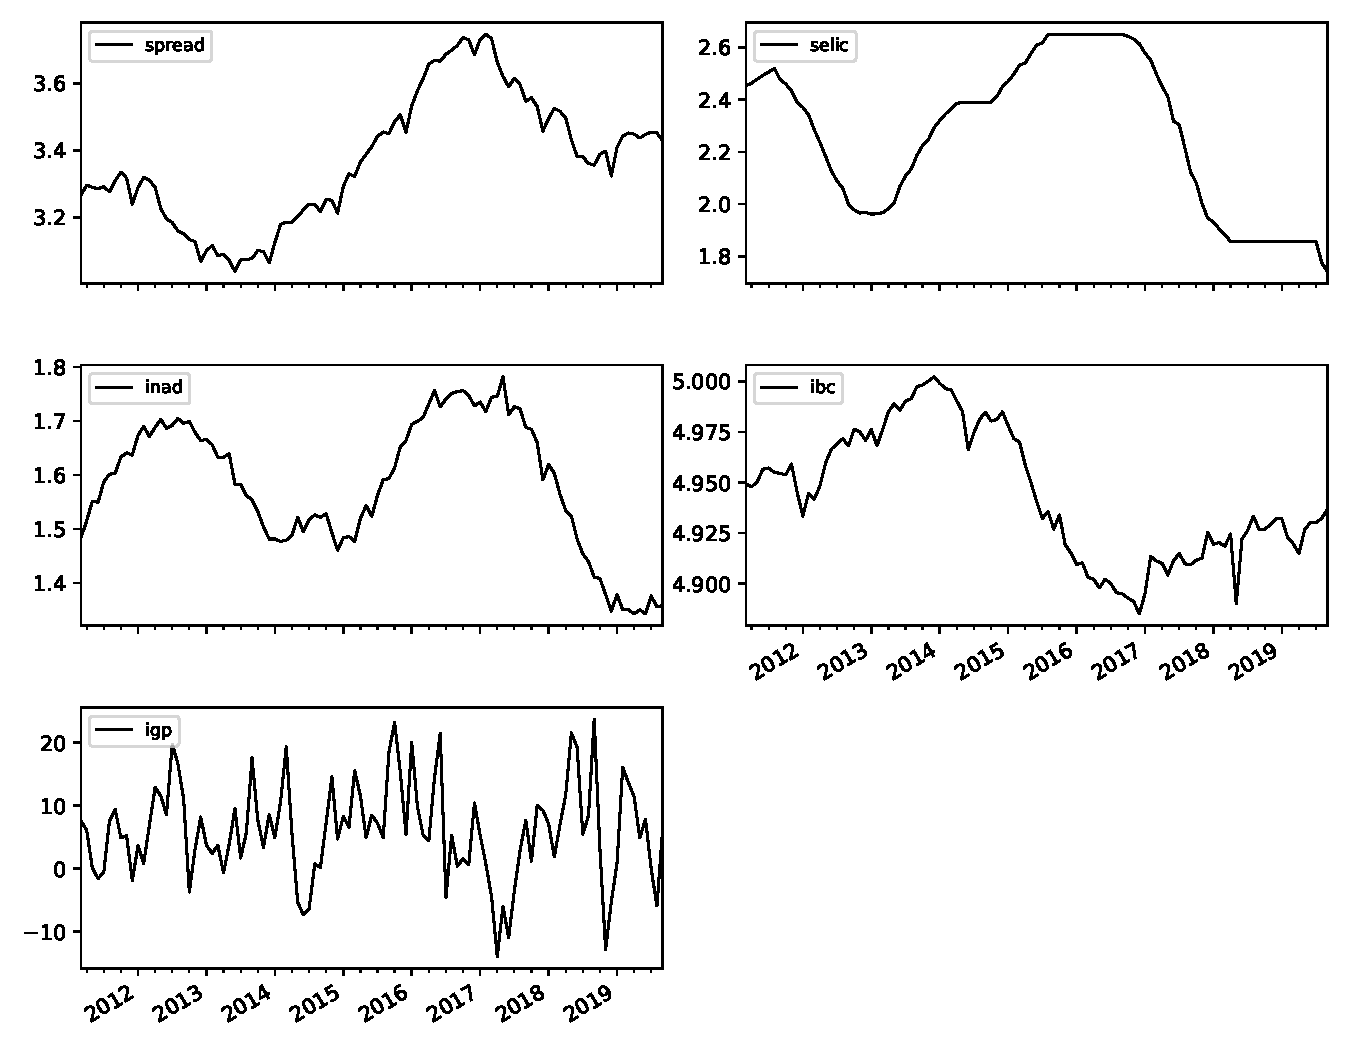
\includegraphics[width = 0.9\textwidth, scale=1]{series_modelo.pdf}
        \label{graficos}
    \end{figure}

   Como determinantes do spread bancário, foram consideradas as variáveis taxa básica de juros (selic), inadimplência (inad), atividade econômica (ibc) e inflação (igp), como expresso pela equação abaixo:

   \begin{equation}
       \label{equacao_modelo}
       \text{spread}_t = \beta_0 + \beta_1 \text{selic}_t + \beta_2 \text{inad}_t + \beta_3 \text{ibc}_t + \beta_4 \text{igp}_t + u_t
   \end{equation}

   Tratam-se de séries temporais mensais que cobrem o período de março de 2011 a agosto de 2019, somando 102 observações, que podem ser vistas na \autoref{graficos}.

   Durante todo o capítulo, faz-se uso extensivo do pacote statsmodels do Python, dos autores \textcite{statsmodels}.

   \subsection{Testes de raiz unitária}
   
   Na \autoref{raiz_unitaria} estão compilados os resultados do teste de \textit{Augmented Dickey-Fuller} com o número de defasagens sendo escolhido com base no \textit{Bayesian Information Criterion} (BIC).

    \newcolumntype{C}[1]{>{\centering\arraybackslash}p{#1}}

    \begin{table}[ht]
        \IBGEtab{\caption{Teste Augmented Dickey-Fuller de raiz unitária}\label{raiz_unitaria}}
        {%
            \begin{tabular}{lcccc}
                \midrule
                & \multicolumn{1}{c}{} & \multicolumn{1}{C{3cm}}{Sem drift e sem tendência} & \multicolumn{1}{C{3cm}}{Com drift} & \multicolumn{1}{C{3cm}}{Com tendência} \\
                \midrule
                Variável & Defasagem & \multicolumn{3}{c}{P-valor} \\
                \midrule
                spread*      &         12 &     0.67 &     0.12 &     0.00 \\
                selic        &          4 &     0.23 &     0.61 &     0.79 \\
                ibc          &          0 &     0.59 &     0.68 &     0.75 \\
                inad         &          4 &     0.37 &     0.17 &     0.39 \\
                igp*         &          0 &     0.00 &     0.00 &     0.00 \\
                \midrule
            \end{tabular}
            } 
            {\fonte{Elaboração própria, com base na função adfuller do pacote statsmodels do Python.}\nota{$ \text{H}_0 $: raiz unitária. $ \text{H}_a $: estacionária. \newline * Estacionariedade.}}
    \end{table}

    Nela podemos ver que há forte evidência de estacionariedade para a série igp e de não-estacionariedade para o ibc, em qualquer dos cenários. Há, ainda, evidência de tendência-estacionariedade para o spread. A selic e a inadimplência não foram consideradas estacionárias em qualquer dos cenários.

    A \autoref{pp} apresenta os resultados para o teste de Phillips-Perron, em que somente a variável igp foi diagnosticada como estacionária.

    \begin{table}[ht]
        \IBGEtab{\caption{Teste Phillips-Perron de raiz unitária}\label{pp}}
        {%
            \begin{tabular}{lcccc}
                \midrule
                &           & \multicolumn{1}{C{3cm}}{Sem drift e sem tendência} & \multicolumn{1}{C{3cm}}{Com drift} & \multicolumn{1}{C{3cm}}{Com tendência} \\
                \midrule
                Variável & Defasagem & \multicolumn{3}{c}{P-valor} \\
                \midrule
                spread     &         13 &     0.76 &     0.61 &     0.79 \\
                selic      &         13 &     0.31 &     0.76 &     0.90 \\
                ibc        &         13 &     0.60 &     0.61 &     0.65 \\
                inad       &         13 &     0.54 &     0.57 &     0.72 \\
                igp*        &         13 &     0.00 &     0.00 &     0.00 \\
                \midrule
            \end{tabular}
            } 
            {\fonte{Elaboração própria, com base na função PhillipsPerron do pacote arch do Python.}\nota{$ \text{H}_0 $: raiz unitária. $ \text{H}_a $: estacionária. \newline * Estacionariedade.}}
    \end{table}

    Por fim, na \autoref{kpss} constam os resultados do teste \textit{Kwiatkowski-Phillips-Schmidt-Shin} (KPSS) de estacionariedade, que se distingue por ter como hipótese nula a estacionariedade ao invés da raiz unitária.

    \begin{table}[ht]
        \IBGEtab{\caption{Teste KPSS de estacionariedade}\label{kpss}}
        {%
            \begin{tabular}{lcccc}
                \midrule
                & \multicolumn{2}{C{5cm}}{$ \text{H}_0 $: constante-estacionária} & \multicolumn{2}{C{5cm}}{$ \text{H}_0 $: tendência-estacionária} \\
                \midrule
                Variável & Defasagem & P-valor & Defasagem & P-valor \\
                \midrule
                spread     &          6 &     0.01 &          5 &     0.01 \\
                selic*      &          6 &     0.09 &          6 &     0.01 \\
                ibc        &          5 &     0.01 &          5 &     0.01 \\
                inad*       &          5 &     0.10 &          5 &     0.02 \\
                igp*        &          4 &     0.10 &          4 &     0.10 \\
                \midrule
            \end{tabular}
            } 
            {\fonte{Elaboração própria, com base na função kpss do pacote statsmodels do Python.}\nota{$ H_0 $: estacionariedade. $ H_a $: raiz unitária. \newline * Estacionariedade.}}
    \end{table}

    Ele reforça a evidência de que a variável do igp seja estacionária. Além disso, contrariando os outros testes, encontra evidência de estacionariedade para a variável do inad e selic. Já o ibc continuou como não-estacionário.

    Portanto, a selic e inad foram diagnosticadas como estacionárias somente pelo KPSS\@, sendo provavelmente não-estacionárias. O ibc foi consistentemente diagnosticado como não-estacionário, o mesmo valendo para a estacionariedade do igp.

    Dado estes resultados, é razoável concluir que as variáveis selic, spread, inad e ibc têm raiz unitária. 
    
    O próximo passo agora é investigar se há co-integração entre alguma combinação linear das variáveis spread, selic, inad e ibc, ou seja, se há um equilíbrio de longo prazo entre elas.
    
    Esta é uma hipótese razoável de se fazer, visto possuir um sentido econômico: há uma relação muito próxima entre o spread e a taxa Selic (pelo efeito custo de oportunidade etc.), a inadimplência (efeito custo de crédito) e a atividade econômica (pelo efeito inadimplência, poder de mercado, melhora na percepção de risco etc.).

    \subsection{Teste de co-integração uni-equacional}

    Para isso utilizaremos o teste de Engle-Granger, cujos resultados podem ser vistos na \autoref{coint_resultados}.

    \begin{table}[ht]
        \IBGEtab{\caption{Teste de co-integração}\label{coint_resultados}}
        {%
            \begin{tabular}{lccccccc}
                \midrule
                Atv. Econômica & Tendência & Engle-Granger & P-valor & 1\% & 5\% & 10\% \\
                \midrule
                ibc* & Sim & -5.16 & 0.01 & -5.2 & -4.57 & -4.26 \\
                ibc* & Não & -4.84 & 0.01 & -4.83 & -4.21 & -3.89 \\
                \midrule
            \end{tabular}
            } 
            {\fonte{Elaboração própria, com base na função coint do pacote statsmodels do Python.}\nota{* Co-integração.}}
    \end{table}

    Desses resultados se conclui que há evidência de co-integração ao nível de significância de 5\%, independente do termo de tendência.
    
    \subsection{Modelo uni-equacional de correção de erros}

    Por essa razão, foi utilizada a equação sem tendência para fazer a estimação da relação de equilíbrio de longo prazo. Os resultados estão na \autoref{coint_reg}.

    \begin{table}[!hbt]
        \IBGEtab{\caption{Relação de co-integração}\label{coint_reg}}{%
            \centering
            \label{}
            \begin{tabular}{@{\extracolsep{20pt}}lcc}
                \midrule
                \midrule
                                  & \multicolumn{1}{c}{Variável dependente:} \\
                \cline{2-2}
                                  & spread \\
                \midrule
                Intercept         & 30.2636***       \\
                                  & (1.0014)         \\
                selic             & 0.1619***        \\
                                  & (0.0238)         \\
                inad              & -0.0839          \\
                                  & (0.0596)         \\
                ibc               & -5.4874***       \\
                                  & (0.1967)         \\
                \midrule
                Observações       & 102.0000         \\
                $ R^2 $           & 0.9056           \\
                $ R^2 $ Ajustado  & 0.9027           \\
                Estatística F     & 313.346 (0.000)  \\
                Jarque-Bera       & 1.806 (0.405)    \\
                Dickey-Fuller     & -4.156 (0.001)   \\
                Durbin-Watson     & 0.706            \\
                \midrule
                \midrule
            \end{tabular}
            }{\nota{* $ p<0.1 $; ** $ p<0.05 $; *** $ p<0.01 $. \newline Entre parênteses: nos coeficientes, o desvio-padrão, nas estatísticas, o p-valor.}}
    \end{table}

    Os sinais dos coeficientes são os esperados, apesar de insignificante para a inadimplência. 
    
    Chama atenção também o especialmente alto valor do coeficiente da variável ibc, significando que, no longo prazo, um aumento de 1\% na atividade econômica diminui, em média, o nível do spread em 5.48\%. Analogamente, um aumento de 1\% na selic aumenta em 0.16\% o spread.

    Além disso, como esperado de um termo de equilíbrio, os resíduos dessa regressão apresentam evidência de ser um processo estacionário autorregressivo de ordem 1, como esperado pela teoria \footcite[12]{coint1}, o que é verificado pela estatística de Durbin-Watson entre 0 e 1 e pelo baixo p-valor da estatística de Dickey-Fuller.

    Agora, para observar os efeitos de curto prazo sobre o spread, estimamos o modelo de correção de erros: $ \Delta \textit{spread} = \alpha (\textit{spread} - \hat{\beta_0} - \hat{\beta_1} \textit{selic} -\hat{\beta_2} \textit{inad} + \hat{\beta_3} \textit{igp)}\ +\ \alpha_1 \Delta \textit{selic}\ +\ \alpha_2 \Delta \textit{inad}\ +\ \alpha_3 \Delta \textit{igp} + u_t $.

    A estimação dos coeficientes desta equação são relatados na \autoref{modelo_ecm} abaixo.

    \begin{table}[!hbt]
        \IBGEtab{\caption{Modelo de correção de erros}\label{modelo_ecm}}{%
            \centering
            \label{}
            \begin{tabular}{@{\extracolsep{20pt}}lcc}
                \midrule
                \midrule
                                  & \multicolumn{1}{c}{Variável dependente:} \\
                \cline{2-2}
                                  & spread \\
                \midrule
                equilibrio        & -0.1009*        \\
                                  & (0.0547)        \\
                selic             & 0.2186**        \\
                                  & (0.0936)        \\
                inad              & 0.5216***       \\
                                  & (0.1317)        \\
                ibc               & -0.4502         \\
                                  & (0.4184)        \\
                \midrule
                Observações       & 101.0000        \\
                $ R^2 $           & 0.2862          \\
                $ R^2 $ Ajustado  & 0.2567          \\
                Estatística F     & 9.722 (0.000)   \\
                Jarque-Bera       & 3.023 (0.221)   \\
                Dickey-Fuller     & -8.347 (0.000)  \\
                Durbin-Watson     & 1.781           \\
                \midrule
                \midrule
            \end{tabular}
            }{\nota{* $ p<0.1 $; ** $ p<0.05 $; *** $ p<0.01 $. \newline Entre parênteses: nos coeficientes, o desvio-padrão, nas estatísticas, o p-valor.}}
    \end{table}

    Eles permitem interpretar que, dentro de um mês, 10\% do spread é corrigido quando em desequilíbrio. Além disso, os efeitos de curto prazo foram tais que 1\% de aumento na selic aumenta o spread em 0.21\% e 1\% de aumento na inadimplência aumenta o spread em 0.52\%, ao passo que o efeito de curto prazo da atividade econômica sobre o spread não foi significante.

    Isto sugere que o efeito-inadimplência sobre o spread é melhor explicado pela variável da inadimplência no curto prazo, mas melhor explicado pela atividade econômica no longo prazo.
    
    Este efeito ter sido dominado por ambas, em duas equações, de tal forma a tornar a outra insignificante estatisticamente, indica que elas estão explicando o mesmo efeito. Como podemos ver na literatura, esse não é sempre o caso, relevando tão somente que o efeito inadimplência da atividade econômica preponderou sobre qualquer outro efeito que poderia ter a atividade econômica sobre o spread, como o efeito de diminuí-lo por uma melhora nas expectativas.

    \subsection{Modelo vetorial de correção de erros}

    Neste capítulo serão analisados os resultados do modelo de correção de erros multivariado. Primeiro, a etapa pré-estimação, como foram escolhidos o número do defasagem e o posto de co-integração. Por fim, é feita a análise das funções de impulso-resposta e de decomposição da variância.

    O modelo estimado tem a seguinte forma:

    \begin{equation}
        \Delta y_t = \alpha \beta^{'} y_{t-1}+ \Gamma_1 \Delta y_{t-1} + \cdots + \Gamma_{p} \Delta y_{t-1} + CD_t + u_t \label{vecm_spread}
    \end{equation}

    Onde o vetor $ y_t $ contém as variáveis do spread, selic, inad e ibc.
    
    A matriz $ D_t $, cujos coeficientes estão contidos em $ C $, contém termos determinísticos, tais como intercepto e onze variáveis dummy para controlar pela sazonalidade nas séries, além da variável da inflação como exógena. Não foram incluídos termos determinísticos dentro da relação de co-integração.

    Antes da estimação, porém, é necessário determinar qual o posto da matriz de co-integração e o número de defasagem $ p $ do modelo. É o que será feito nas duas próximas seções.

    \subsubsection{Seleção da ordem de defasagem}

    O número de defasagens foi parcimoniosamente escolhido com base no teste de Portmanteau, ou seja, foi escolhido o menor número de defasagem que evidenciasse ausência de autocorrelação. Com este método, chegou-se ao número de 2 defasagens.

    O resultado do teste pode ser visto na \autoref{portmanteau}, onde pode-se ver que não há evidência de autocorrelação até o lag 12.

    \begin{table}[!hbt]
        \IBGEtab{\caption{Teste de Portmanteau}\label{portmanteau}}{%
        \begin{tabular}{cccc}
            \toprule
            Estatística de teste & Valor crítico & P-valor & Graus de liberdade  \\
            \midrule
            170.4          &          186.1          &      0.203       &     156      \\
            \bottomrule
        \end{tabular}
        }{\nota{$ \text{H}_0 $: autocorrelação serial até defasagem 12 é zero.}}
    \end{table}

    \subsubsection{Ordenação das variáveis}

    Como se sabe, a ordenação das variáveis do modelo é crucial para a análise das funções de resposta ao impulso ortogonal e da decomposição da variância, tanto que vale um capítulo para esclarecer que cuidados foram tomados em relação a isso.

    Na literatura empírica, é comum ordenar as variáveis pelo critério de exogeneidade, isto é, da mais exógena para a mais endógena, devido à decomposição de Cholesky resultar em uma matriz triangular inferior. Por exemplo, em \textcite{oreiro} isto é feito com a ajuda de testes de causalidade de Granger.

    No entanto, \textcite[61]{lutkepool} não advoga qualquer ferramenta estatística para essa decisão, tendo de ser tomada analiticamente. Ainda segundo ele, a ordem teria de ser tal que a primeira variável seja a única com o potencial de afetar contemporaneamente todas as outras, com a segunda podendo afetar todas exceto a primeira, a terceira, todas exceto a primeira e segunda etc.

    Com isso em mente, a ordem foi decidida teoricamente: assumindo que a taxa Selic afeta contemporaneamente todas as outras variáveis no sistema, sem ser por elas afetada contemporaneamente, é uma razoável candidata como primeiro variável. Seguida da inadimplência, que influenciaria instantaneamente a atividade econômica e o spread, mas não a taxa Selic. Depois, a atividade econômica, que afetaria a Selic e a inadimplência com no mínimo uma defasagem e, por fim, o spread, que não influenciaria nenhuma das outras contemporaneamente, mas sendo somente por todas elas influenciado.

    \subsubsection{Teste de Johansen}

    Os testes de Johansen aplicados ao modelo VECM de ordem 2 suportam a evidência de uma relação de co-integração no sistema, como pode ser visto nas tabelas \autoref{johansen_max_eig} e \autoref{johansen_trace}.

 \begin{table}[hbt]
     \begin{subtable}{.5\linewidth}
         \IBGEtab{\caption{Teste de Johansen de máximo autovalor}\label{johansen_max_eig}}{%
             \begin{tabular}{cccc}
                 \midrule
                 r\_0 & r\_1 & Estatística de teste & Valor Crítico \\
                 \midrule
                 0 &             1 &                   48.51 &                   27.59  \\
                 1 &             2 &                   14.62 &                   21.13  \\
                 \midrule
             \end{tabular}
             }{\nota{$ \text{H}_0 $: $ r =  r_0 $. $ \text{H}_a $: $ r = r_0 + 1 $}}
     \end{subtable}%
     \begin{subtable}{.5\linewidth}
         \IBGEtab{\caption{Teste de Johansen de traço}\label{johansen_trace}}{%
             \begin{tabular}{cccc}
                 \midrule
                 r\_0 & r\_1 & Estatística de teste & Valor Crítico \\
                 \midrule
                 0 &             4 &                   69.12 &                   47.85  \\
                 1 &             4 &                   20.61 &                   29.80  \\
                 \midrule
             \end{tabular}
             }{\nota{$ \text{H}_0 $: $ r =  r_0 $. $ \text{H}_a $: $ r_0 < r < 4 $}}
     \end{subtable}%
 \end{table}

    Nas duas, rejeita-se a hipótese nula de que não há qualquer relação de co-integração, para, em seguida, ser feito o teste sob a hipótese nula de que há uma relação de co-integração, e, não sendo possível rejeitá-la, concluímos que há uma relação de co-integração.

    Os coeficientes estimados do vetor co-integrante e da \textit{loading matrix} podem ser vistos na \autoref{resultados_coint}. 
    
    \begin{table}[!hbt]
        \IBGEtab{\caption{Coeficientes estimados da relação de longo prazo}\label{resultados_coint}}{%
            \begin{tabular}{llcccccc}
                \centering
                &                     & Coeficiente          & Desvio Padrão    & Z          & P$> |$z$|$           & [0.025          & 0.975]  \\
                \midrule
                spread    & $ \hat{\alpha_1}  $        &      -0.0764         &        0.031     &    -2.463  &         0.014        &       -0.137    &       -0.016     \\
                selic     & $ \hat{\alpha_2}  $        &      -0.0302         &        0.035     &    -0.863  &         0.388        &       -0.099    &        0.038     \\
                ibc       & $ \hat{\alpha_3}  $        &      -0.0362         &        0.014     &    -2.518  &         0.012        &       -0.064    &       -0.008     \\
                inad      & $ \hat{\alpha_4}  $        &      -0.1603         &        0.026     &    -6.182  &         0.000        &       -0.211    &       -0.109     \\
                \midrule
                spread   & $ \hat{\beta_1}  $         &       1.0000         &            0     &         0  &         0.000        &        1.000    &        1.000     \\
                selic    & $ \hat{\beta_2}  $         &      -0.4674         &        0.040     &   -11.783  &         0.000        &       -0.545    &       -0.390     \\
                ibc      & $ \hat{\beta_3}  $         &       5.2031         &        0.228     &    22.773  &         0.000        &        4.755    &        5.651     \\
                inad     & $ \hat{\beta_4}  $         &       0.5153         &        0.083     &     6.185  &         0.000        &        0.352    &        0.679     \\
                \midrule
            \end{tabular}
            }{}
    \end{table}

    As estimativas são muito similares às que vimos na \autoref{coint_reg}, exceto pelo agora significativo coeficiente da inadimplência, implicando que um aumento de 1\% na inadimplência diminuiria o spread em 0.51\%, em média, o que é inesperado e provavelmente denuncia um viés de variável omitida. De modo similar, um aumento de 1\% na selic aumentaria o spread em 0.46\% e um aumento de 1\% no ibc faria diminuir o spread em 5.2\%.

    Ainda de acordo com esses resultados, as equações que mais se auto-corrigem aos desvios em relação ao equilíbrio são, em ordem, a da inadimplência, spread, ibc e selic, apesar do coeficiente da última não ser significativamente diferente de 0.

    \subsubsection{Funções de Impulso-Resposta}

    Neste capítulo serão interpretados os resultados da estimação com base nas funções de resposta da variável spread a um impulso nas diferentes variáveis do sistema. Os gráficos para as funções como um todo podem ser encontrados no anexo.

    Na \autoref{irf_spread} estão os gráficos da função de impulso-resposta com período que se estendem até 24 meses.
    
    \begin{figure}[h!bt]
        \caption{Função de impulso-resposta (spread)}
        \begin{subfigure}[t]{.5\linewidth}
            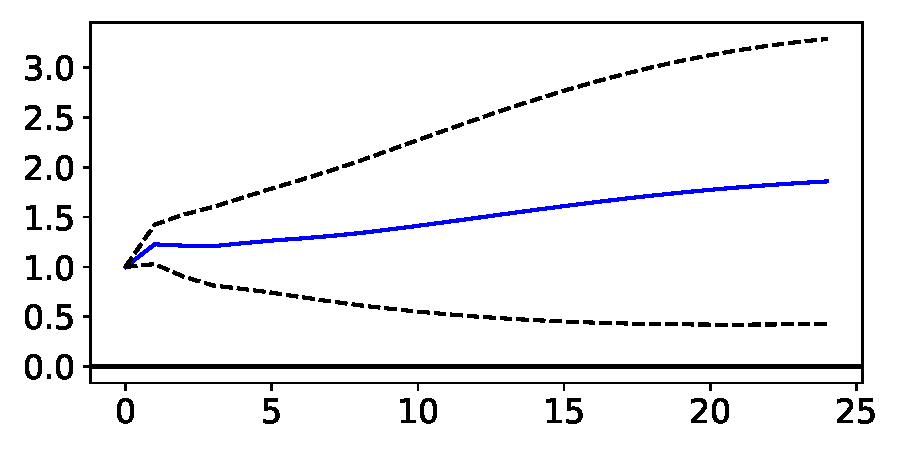
\includegraphics[width = \textwidth, scale=1]{irf/spread_spread.pdf}
            \caption{Impulso: spread}
        \end{subfigure}
        \begin{subfigure}[t]{.5\linewidth}
            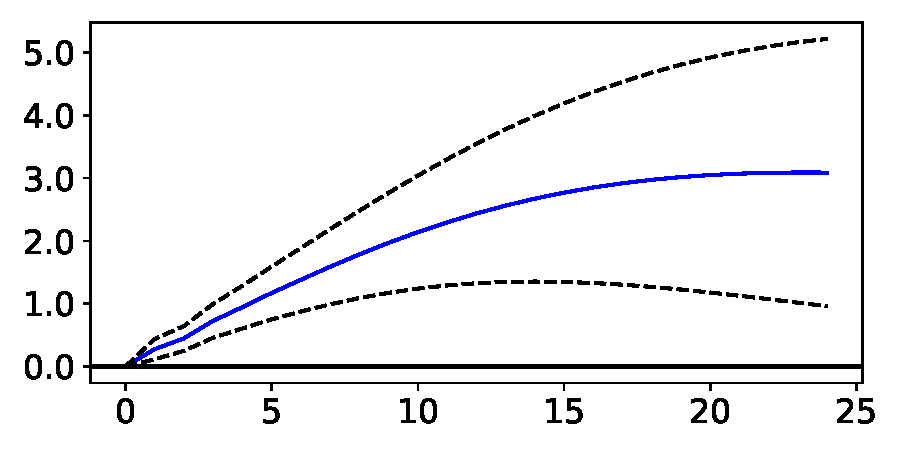
\includegraphics[width = \textwidth, scale=1]{irf/spread_selic.pdf}
            \caption{Impulso: selic}
        \end{subfigure}
        \begin{subfigure}[t]{.5\linewidth}
            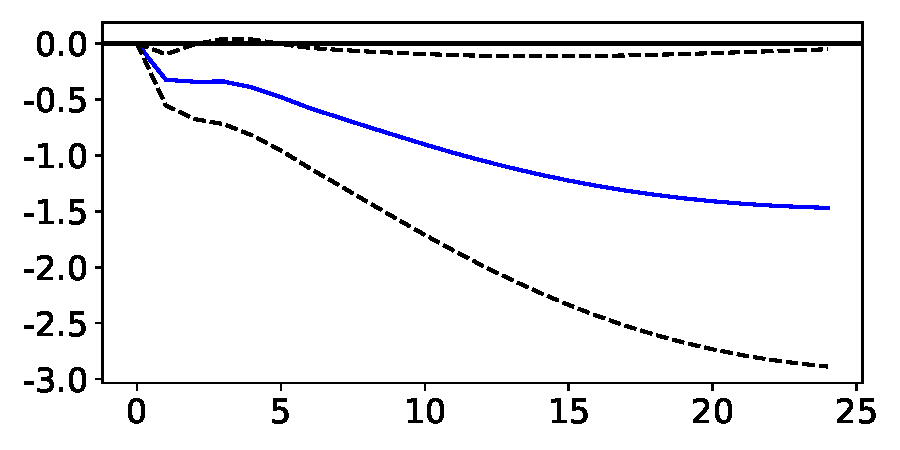
\includegraphics[width = \textwidth, scale=1]{irf/spread_inad.pdf}
            \caption{Impulso: inad}
        \end{subfigure}
        \begin{subfigure}[t]{.5\linewidth}
            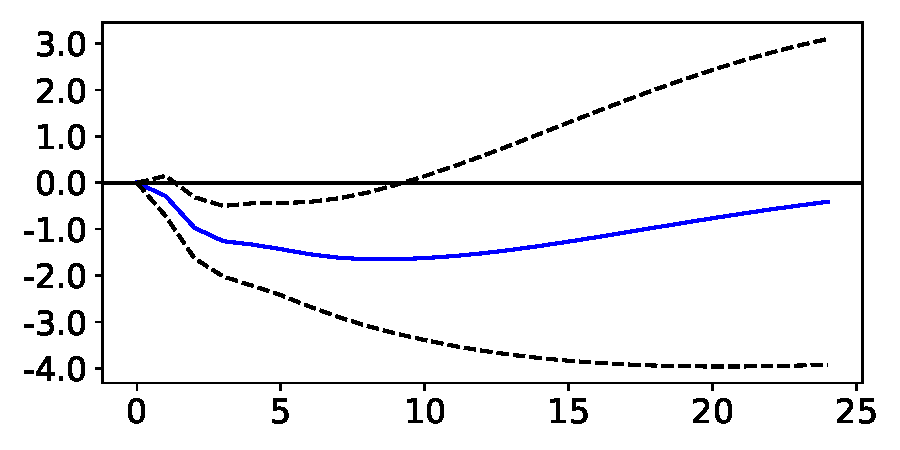
\includegraphics[width = \textwidth, scale=1]{irf/spread_ibc.pdf}
            \caption{Impulso: ibc}
        \end{subfigure}
        \label{irf_spread}
        \legend{Fonte: Elaboração própria, com base no pacote statsmodels.}
    \end{figure}

    Nela podemos constatar que, pela estimação, um impulso na taxa básica de juros causa um aumento persistente no spread, que só vem se estabilizar em mais ou menos 2 anos. E ainda que um impulso na atividade econômica diminuiria o spread com alguns meses de defasagem, sendo o sinal insignificante para período mais longos. Já um impulso na inadimplência teria o efeito de diminuir o spread, o que é inesperado e provavelmente se deve a um viés de variável omitida ou pelos resíduos não serem ortogonais.

    A seguir, serão mostradas as funções de resposta ao impulso ortogonal, com base na ordenação já mencionada: selic, inad, ibc e spread.

    \begin{figure}[h!bt]
        \label{irf_spread_ortogonal}
        \caption{Função de impulso-resposta ortogonal (spread)}
        \begin{subfigure}[t]{.5\linewidth}
            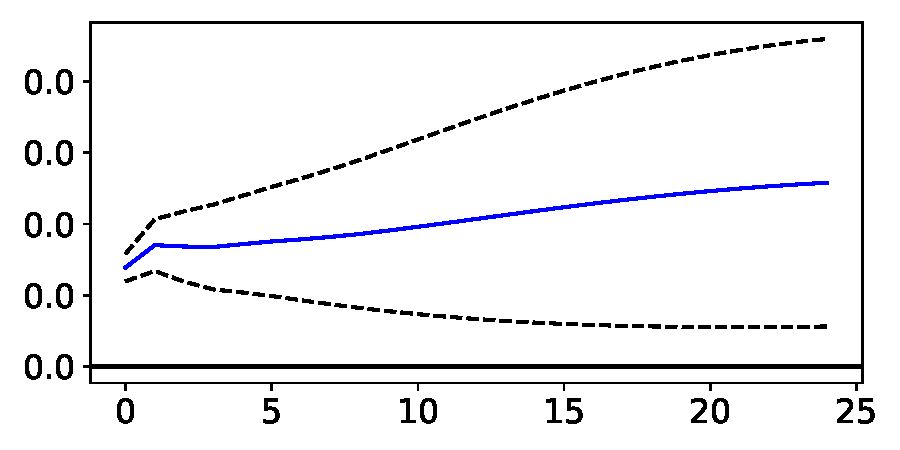
\includegraphics[width = \textwidth, scale=1]{irf/orth_spread_spread.pdf}
            \caption{Impulso: spread}
        \end{subfigure}
        \begin{subfigure}[t]{.5\linewidth}
            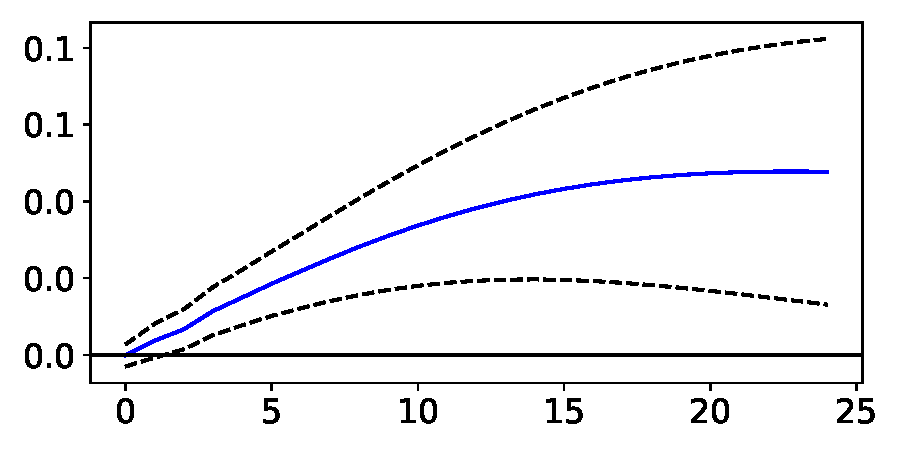
\includegraphics[width = \textwidth, scale=1]{irf/orth_spread_selic.pdf}
            \caption{Impulso: selic}
        \end{subfigure}
        \begin{subfigure}[t]{.5\linewidth}
            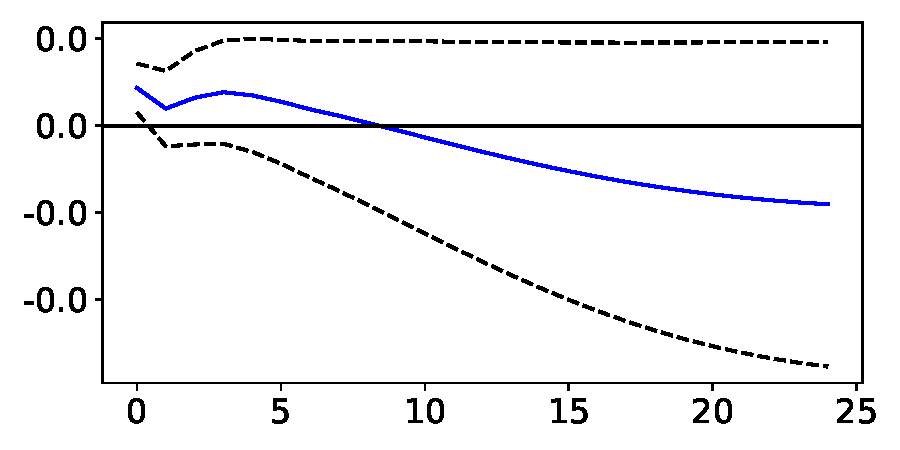
\includegraphics[width = \textwidth, scale=1]{irf/orth_spread_inad.pdf}
            \caption{Impulso: inad}
        \end{subfigure}
        \begin{subfigure}[t]{.5\linewidth}
            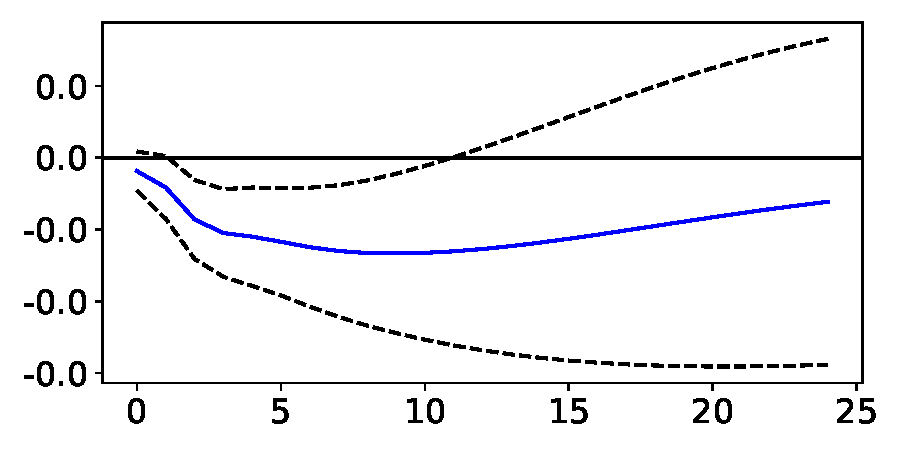
\includegraphics[width = \textwidth, scale=1]{irf/orth_spread_ibc.pdf}
            \caption{Impulso: ibc}
        \end{subfigure}
    \end{figure}





\newpage
\printbibliography

\end{document}
